

\documentclass[11pt,compress,t,notes=noshow]{beamer}

\usepackage[english]{babel}
\usepackage{dsfont}
\newcommand\bmmax{2}
\usepackage{bm}
\usepackage{bbm}
\usepackage{verbatim}
\usepackage{amsmath}
\usepackage{amsfonts}
\usepackage{csquotes}
\usepackage{multirow}
\usepackage{longtable}
\usepackage{enumerate}
\usepackage[absolute,overlay]{textpos}
\usepackage{psfrag}
\usepackage{algorithm}
\usepackage{algorithmicx}
\usepackage{algpseudocode}
\usepackage{eqnarray}
\usepackage{multimedia}
\usepackage{media9}
\usepackage{arydshln}
\usepackage{tabularx}
\usepackage{placeins}
\usepackage{tikz}
\usepackage{setspace}
\usepackage{wrapfig}
\usepackage{tcolorbox}
\usepackage[export]{adjustbox}
\usepackage{siunitx}
\usetikzlibrary{shapes,arrows,automata,positioning,calc}
\tikzset{
  %Define standard arrow tip
  >=stealth',
  %Define style for boxes
  punkt/.style={
    rectangle,
    rounded corners,
    draw=black, very thick,
    text width=6.5em,
    minimum height=2em,
    text centered},
  % Define arrow style
  pil/.style={
    ->,
    thick,
    shorten <=2pt,
    shorten >=2pt,}
}
\usepackage{subfig}

%new environments

\newenvironment{vbframe}  %frame with breaks and verbatim
{
 \begin{frame}[containsverbatim,allowframebreaks]
}
{
\end{frame}
}

\newenvironment{vframe}  %frame with verbatim without breaks (to avoid numbering one slided frames)
{
 \begin{frame}[containsverbatim]
}
{
\end{frame}
}

\newenvironment{blocki}[1]   % itemize block
{
 \begin{block}{#1}\begin{itemize}
}
{
\end{itemize}\end{block}
}

\newenvironment{fragileframe}[2]{  %fragile frame with framebreaks
\begin{frame}[allowframebreaks, fragile, environment = fragileframe]
\frametitle{#1}
#2}
{\end{frame}}


\newcommand{\myframe}[2]{  %short for frame with framebreaks
\begin{frame}[allowframebreaks]
\frametitle{#1}
#2
\end{frame}}

\newcommand{\remark}[1]{
  \textbf{Remark:} #1
}

%%%%%%%%%%%%%%%%%%%%%%%%%%%%%%%%%%%%%%%%%%%%%%%%%%%%%%%%%%%%%%%%%%%%%%%%%%%%%%%

% basic latex stuff
\newcommand{\pkg}[1]{{\fontseries{b}\selectfont #1}} %fontstyle for R packages
\newcommand{\lz}{\vspace{0.5cm}} %vertical space
\newcommand{\dlz}{\vspace{1cm}} %double vertical space
\newcommand{\oneliner}[1] % Oneliner for important statements
{\begin{block}{}\begin{center}\begin{Large}#1\end{Large}\end{center}\end{block}}


%\usetheme{lmu-lecture}
\usepackage{../style/lmu-lecture}

\let\code=\texttt
\let\proglang=\textsf

\setkeys{Gin}{width=0.9\textwidth}


\title{Deep Learning}
\author{Mina Rezaei}
\institute{Department of Statistics -- LMU Munich}
\date{Winter Semester 2021}

\setbeamertemplate{frametitle}{\expandafter\uppercase\expandafter\insertframetitle}

%\begin{document}
%\sloppy
%\end{document}

 
\input{../../latex-math/basic-math}
\input{../../latex-math/basic-ml}
\input{../../latex-math/ml-nn}

\begin{document}


\lecturechapter{6}{Important Types of Convolutions}
\lecture{Deeplearning}
%%%%%%%%%%%%%%%%%%%%%%%%%%%%%%%%%%%%%%%%

\begin{frame}
\frametitle{Lecture outline}
\tableofcontents
\end{frame}

%%%%%%%%%%%%%%%%%%%%%%%%%%%%%%%%%%%%%%%%

\section{1D Convolutions}

\begin{vbframe}{1D Convolutions}
\textbf{Data situation}: Sequential, 1-dimensional tensor data. 

\begin{itemize}
\item Data consists of tensors with shape [depth, xdim]
\item Depth $1$ (single-channel):
    \begin{itemize}
        \item Univariate time series, e.g. development of a single stock price over time
        \item Functional / curve data
    \end{itemize}
\item Depth $> 1$ (mutli-channel):
    \begin{itemize}
        \item Multivariate time series, e.g.
        \begin{itemize}
            \item Movement data measured with multiple sensors for human activity recognition
            \item Temperature and humidity in weather forecasting
        \end{itemize}
        \item Text encoded as character-level one-hot-vectors 
    \end{itemize}
\end{itemize}

$\to$ Convolve the data with a 1D-kernel

\end{vbframe}
%%%%%%%%%%%%%%%%%%%%%%%%%%%%%%%%%%%%%%%%%%%%

\begin{vbframe}{1D Convolutions -- Operation}
    \begin{figure}
        \centering
        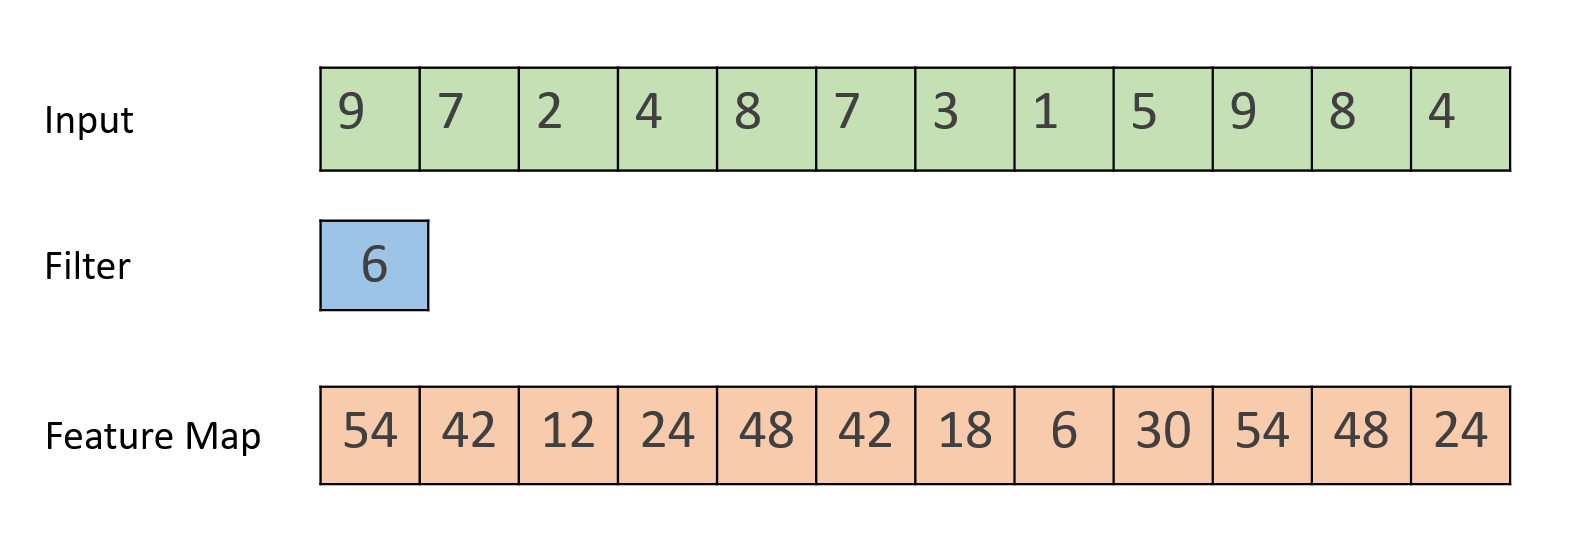
\includegraphics[width=10cm]{plots/1dconv.png}
        \caption{Illustration of 1D movement data with depth $1$ and filter size $1$. }
    \end{figure}
\framebreak
    \begin{figure}
        \centering
        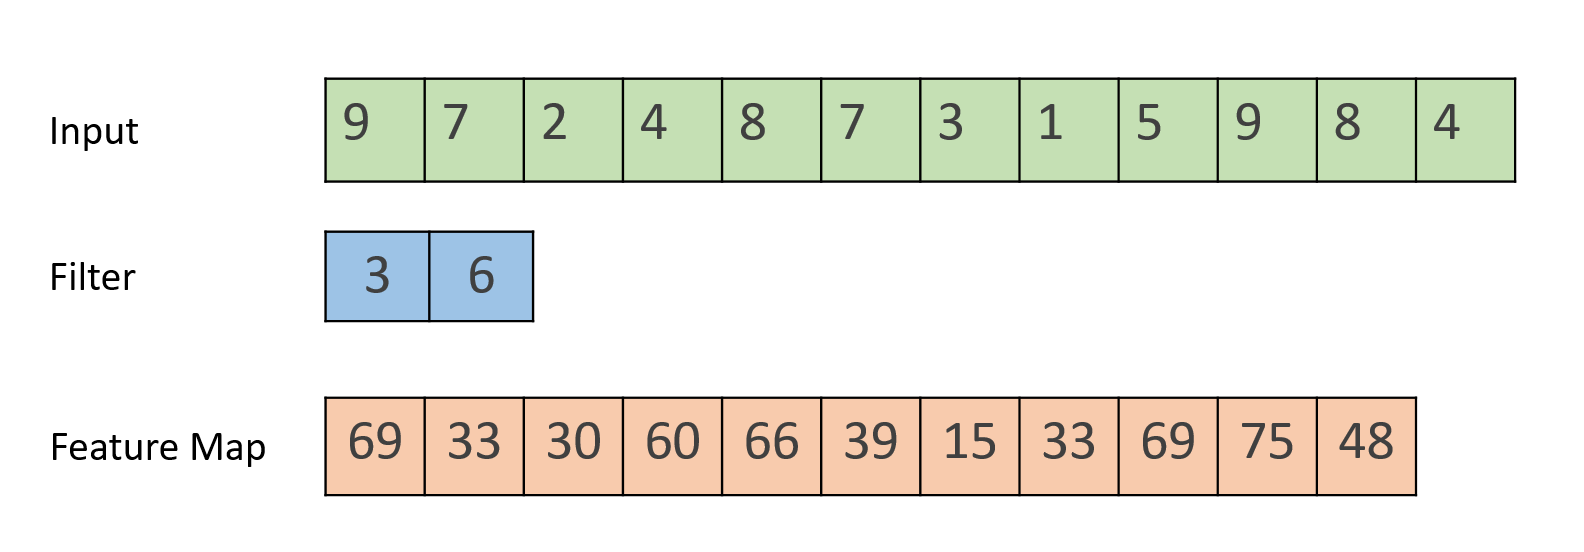
\includegraphics[width=10cm]{plots/1dconv2.png}
        \caption{Illustration of 1D movement data with depth $1$ and filter size $2$. }
    \end{figure}
\end{vbframe}
%%%%%%%%%%%%%%%%%%%%%%%%%%%%%%%%%%%%%%%%%%%%%%%%%%

\begin{vbframe}{1D Convolutions -- Sensor data}
    \begin{figure}
        \centering
        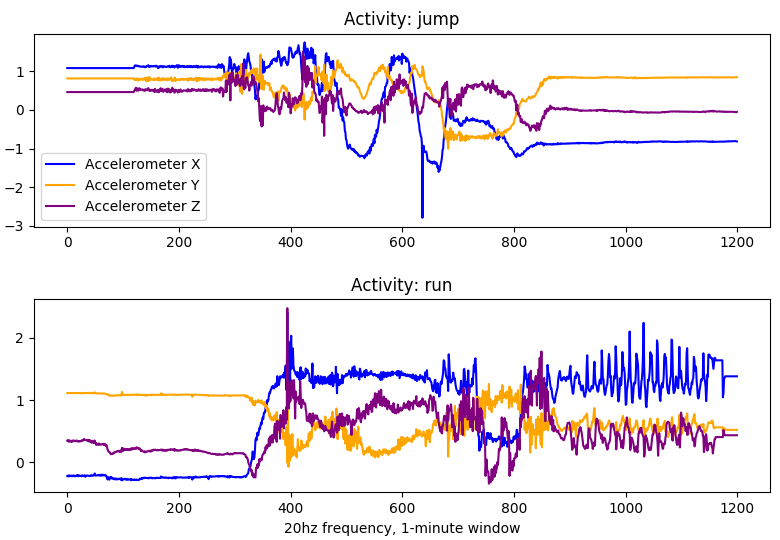
\includegraphics[width=9cm]{plots/05_conv_variations/1d/HAR.png}
        \caption{Illustration of 1D movement data with depth $3$ measured with an accelerometer sensor belonging to a human activity recognition task. }
    \end{figure}
\framebreak
    \begin{figure}
        \centering
        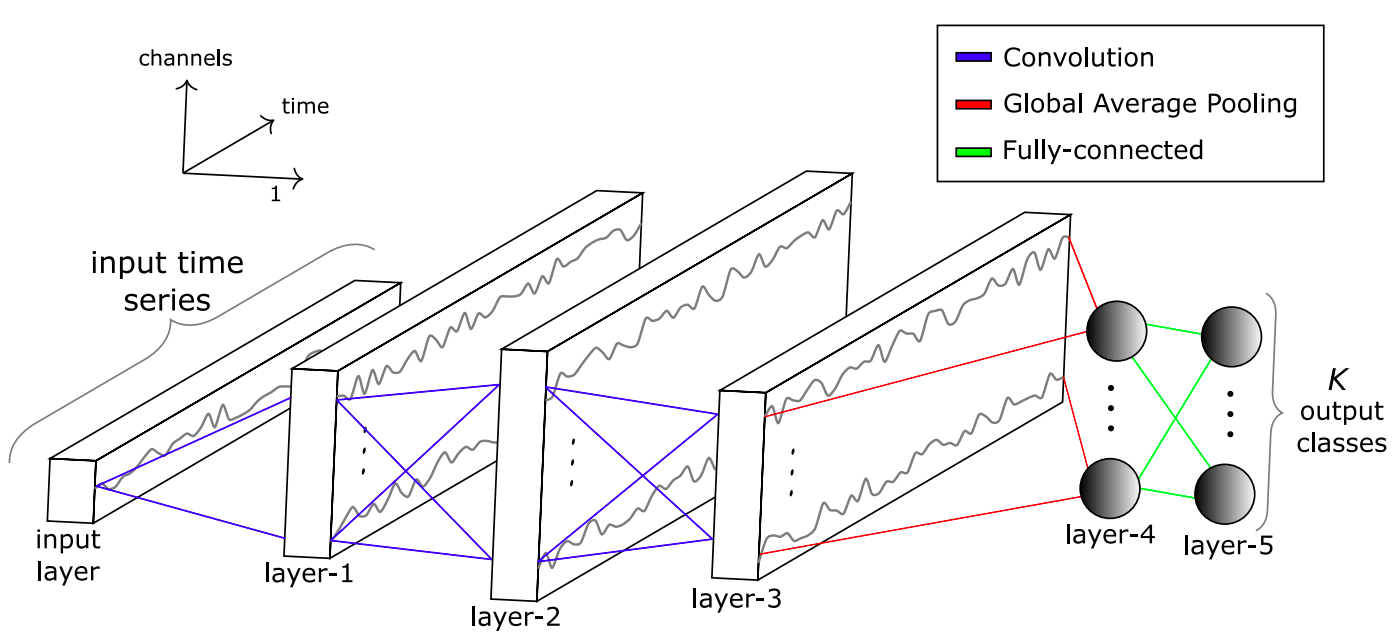
\includegraphics[width=10cm]{plots/05_conv_variations/1d/deep_tsc.png}
        \caption{Time series classification with 1D CNNs and global average pooling (explained later). An input time series is convolved with 3 CNN layers, pooled and fed into a fully connected layer before the final softmax layer. This is one of the classic time series classification architectures.}
    \end{figure}
\end{vbframe}
%%%%%%%%%%%%%%%%%%%%%%%%%%%%%%%%%%%%%%%%%%%%%%%%%%%%%

\begin{vbframe}{1D Convolutions -- Text mining}
    \begin{itemize}
        \item 1D convolutions also have an interesting application in text mining.
        \item For example, they can be used to classify the sentiment of text snippets such as yelp reviews.
    \end{itemize}
    \begin{figure}
        \centering
        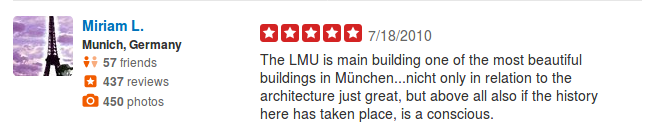
\includegraphics[width=12cm]{plots/05_conv_variations/1d/yelp_lmu.png}
        \caption{Sentiment classification: can we teach the net that this a positive review?}
    \end{figure}
\end{vbframe}
%%%%%%%%%%%%%%%%%%%%%%%%%%%%%%%%%%%%%%%%%%%%%%%%

\frame{
\frametitle{1D Convolutions -- Text mining}    
    \center
    \only<1>{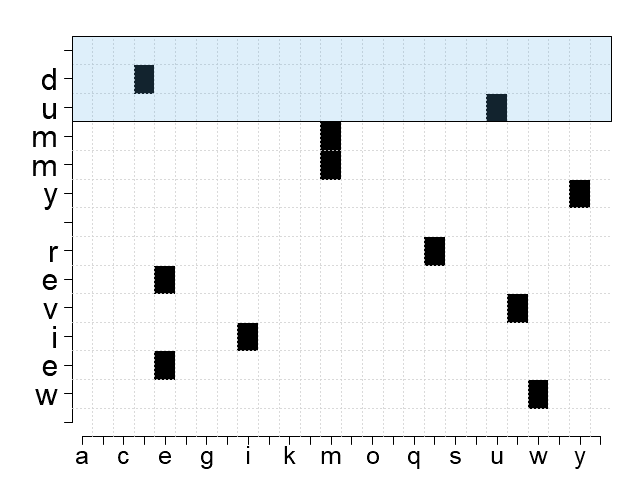
\includegraphics[width=5cm]{plots/text_encoding/1_encoded_text.png}}%
    \only<2>{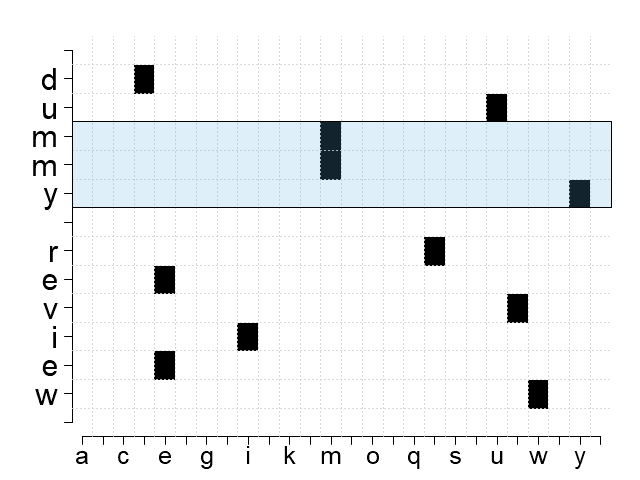
\includegraphics[width=9cm]{plots/text_encoding/4_encoded_text.png}}%
    \only<3>{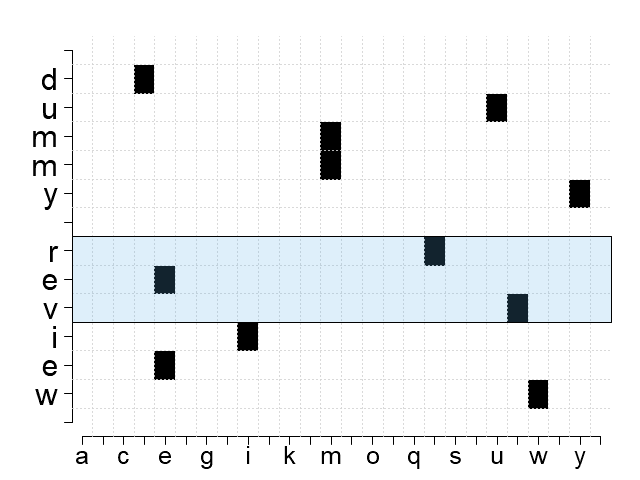
\includegraphics[width=9cm]{plots/text_encoding/8_encoded_text.png}}%
    \only<4>{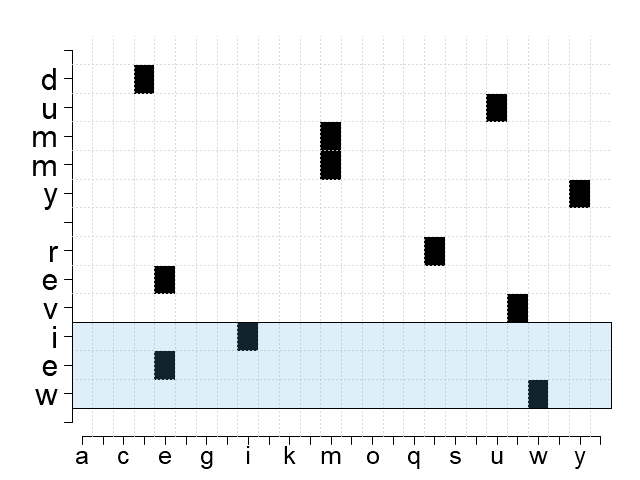
\includegraphics[width=9cm]{plots/text_encoding/11_encoded_text.png}}%
    \\
    % \only<1>{1D convolution of text that was encoded on a character-level. The data is represented as 1D signal with channel size = size of the alphabet as shown in \cite{20}. The temporal dimension is shown as the y dimension for illustrative purposes. The 1D-kernel (blue) convolves the input in the temporal y-dimension yielding a 1D feature vector}  
    \begin{itemize}
        \only<1>{\item We use a given alphabet to encode the text reviews (here: \textit{\enquote{dummy review}}).}
        \only<1>{\item Each character is transformed into a one-hot vector. The vector for character \textit{d} contains only 0's at all positions except for the 4th position.}
        \only<1>{\item The maximum length of each review is set to 1014: shorter texts are padded with spaces (zero-vectors), longer texts are simply cut.}
        \only<2>{\item The data is represented as 1D signal with \emph{depth = size of the alphabet} .}
        \only<3>{\item The temporal dimension is shown as the y dimension for illustrative purposes. }
        \only<4>{\item The 1D-kernel (blue) convolves the input in the temporal y-dimension yielding a 1D feature vector. }
    \end{itemize}
}
%%%%%%%%%%%%%%%%%%%%%%%%%%%%%%%%%%%%%%%%%%%%%%%%

\begin{vbframe}{Advantages of 1D Convolutions}
A few advantages of $1 \times 1$ convolutions are:
   \begin{itemize}
     \item Dimensionality reduction for efficient computations
     \item Efficient low dimensional embedding, or feature pooling     
     \item Applying nonlinearity again after convolution
     \end{itemize}
The first two advantages can be observed in the previous examples. After 1 $\times$ 1 convolution, we significantly reduce the dimension depth-wise. Say if the original input has 200 channels, the 1  $\times$ 1 convolution will embed these channels (features) into a single channel. 

The third advantage comes in as after the 1  $\times$ 1 convolution, non-linear activation such as ReLU can be added. The non-linearity allows the network to learn more complex function.

\end{vbframe}

%%%%%%%%%%%%%%%%%%%%%%%%%%%%%%%%%%%%%%%%%%%%%%%
\section{2D Convolutions}
%%%%%%%%%%%%%%%%%%%%%%%%%%%%%%%%%%%%%%%%%%

\begin{vbframe}{2D Convolutions}

The basic idea behind a 2D convolution is sliding a small window (called a "kernel/filter") over a larger 2D array, and performing a dot product between the filter elements and the corresponding input array elements at every position.
    \begin{figure}
        \centering
        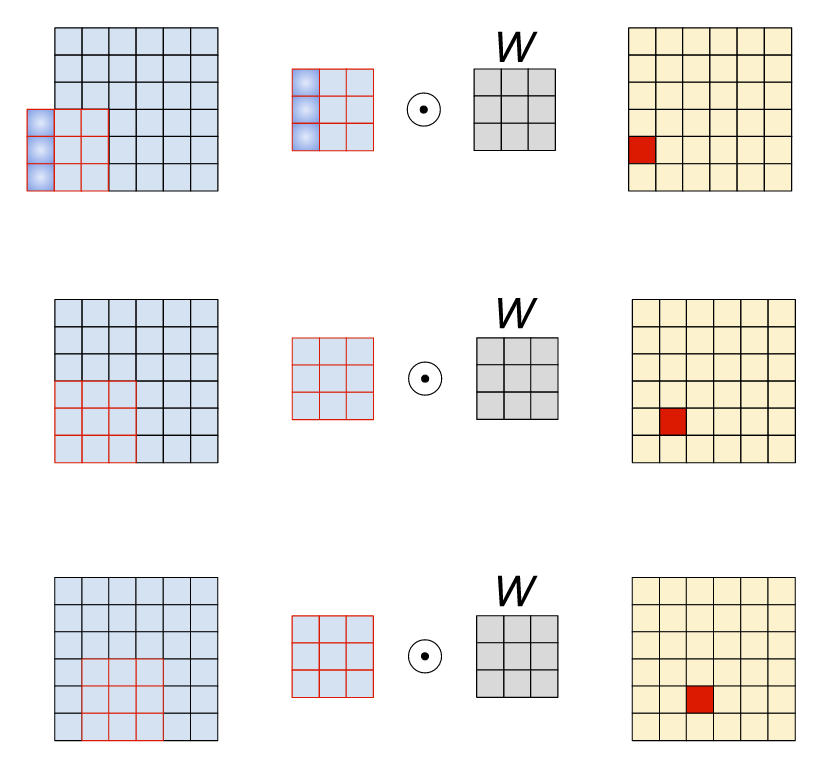
\includegraphics[width=4cm]{plots/05_conv_variations/2d/2dconv.png}
        \caption{\tiny Here's a diagram demonstrating the application of a 3$\times$3 convolution filter to a 6$\times$6 array, in 3 different positions. W is the filter, and the yellow-ish array on the right is the result; the red square shows which element in the result array is being computed.\href{https://eli.thegreenplace.net/2018/depthwise-separable-convolutions-for-machine-learning/}{here}.}
    \end{figure}
\end{vbframe}
%%%%%%%%%%%%%%%%%%%%%%%%%%%%%%%%%%%%%%%%%%%%%%

\frame{
\frametitle{2D Convolutions -- Example}  
    \center
    \only<1>{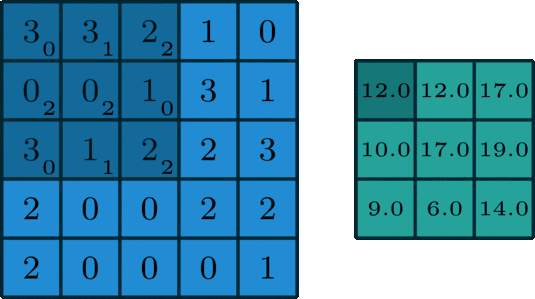
\includegraphics[width=5cm]{plots/05_conv_variations/2d/2dconv-0.png}}%
    \only<2>{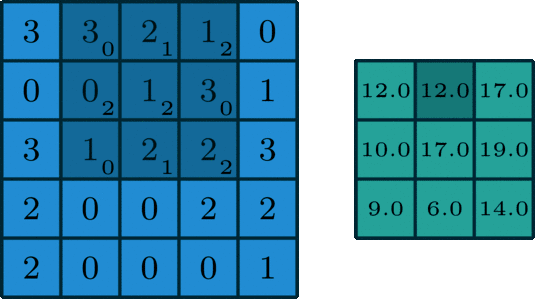
\includegraphics[width=5cm]{plots/05_conv_variations/2d/2dconv-1.png}}%
    \only<3>{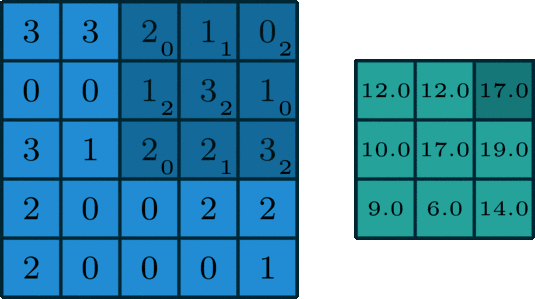
\includegraphics[width=5cm]{plots/05_conv_variations/2d/2dconv-2.png}}%
    \only<4>{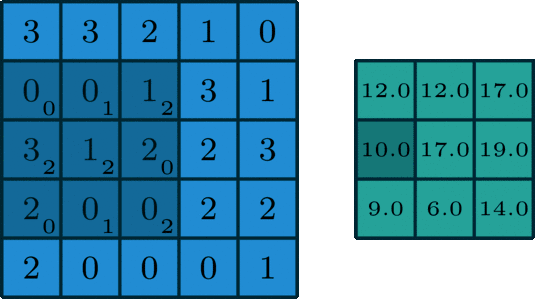
\includegraphics[width=9cm]{plots/05_conv_variations/2d/2dconv-3.png}}%
    \only<5>{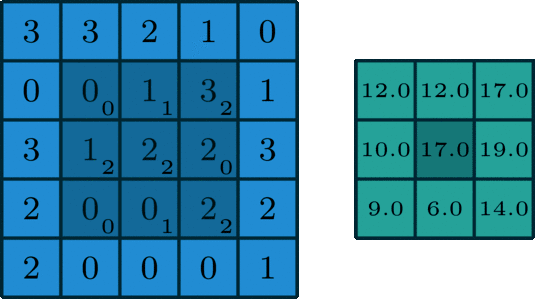
\includegraphics[width=9cm]{plots/05_conv_variations/2d/2dconv-4.png}}%
    \only<6>{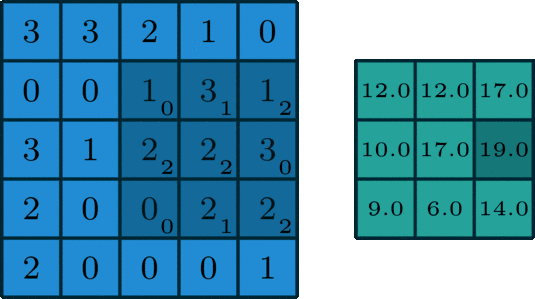
\includegraphics[width=9cm]{plots/05_conv_variations/2d/2dconv-5.png}}%
    \only<7>{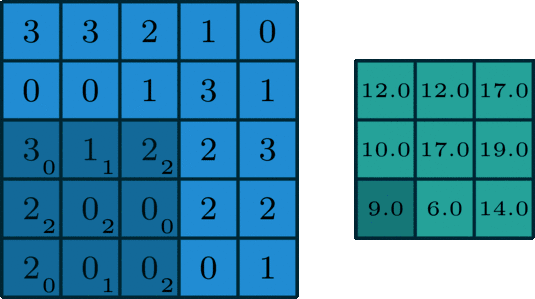
\includegraphics[width=9cm]{plots/05_conv_variations/2d/2dconv-6.png}}%
    \only<8>{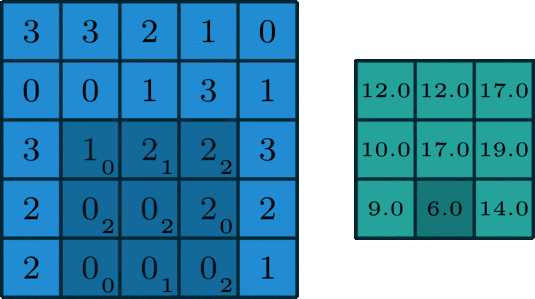
\includegraphics[width=9cm]{plots/05_conv_variations/2d/2dconv-7.png}}%
    \only<9>{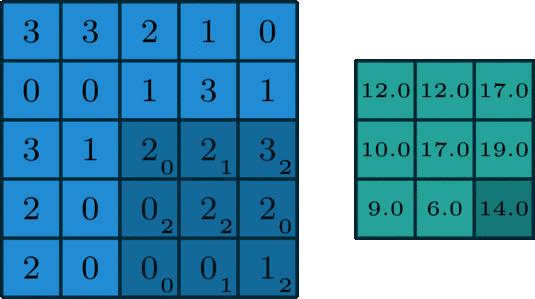
\includegraphics[width=9cm]{plots/05_conv_variations/2d/2dconv-8.png}}%
 \\
    \begin{itemize}
        \only<1>{\item In Deep Learning, convolution is the element-wise multiplication and addition.}
        \only<1>{\item For an image with 1 channel, the convolution is demonstrated in the figure below. Here the filter is a 3$\times$3 matrix with element [[0, 1, 2], [2, 2, 0], [0, 1, 2]].}
        \only<2>{\item The filter is sliding through the input.}
        \only<3>{\item Each sliding position ends up with one number. The final output is then a 3 $\times$ 3 matrix.}
        \only<4>{\item Notice that stride is 1 and padding is 0 in this example.}
        \only<5>{\item We move/convolve filter on input neurons to create a feature maps.}
        \only<6>{\item and ...}
        \only<7>{\item and ...}
        \only<8>{\item and ...}
        \only<9>{\item and at the end we have a 3 $\times$ 3 matrix of feature map!}
    \end{itemize}
}

%%%%%%%%%%%%%%%%%%%%%%%%%%%%%%%%%%%%%%%%%%%%%%%%%%%%

\section{3D Convolutions}

\begin{vbframe}{3D Convolutions}

\textbf{Data situation}: 3-dimensional tensor data.

    \begin{itemize}
        \item Data consists of tensors with shape [depth, xdim, ydim, zdim].
        \item Dimensions can be both temporal (e.g. video frames) or spatial (e.g. MRI)
        \item Examples:
        \begin{itemize}
            \item Human activity recognition in video data
            \item Disease classification or tumor segmentation on MRI scans
        \end{itemize}
    \end{itemize}

\textbf{Solution}: Move a 3D-kernel in $x$, $y$ and $z$ direction to capture all important information.

\end{vbframe}
%%%%%%%%%%%%%%%%%%%%%%%%%%%%%%%%%%%%%%%%%%%%%%%%
\begin{vbframe}{3D Convolutions -- Data}
    \begin{figure}
        \centering
        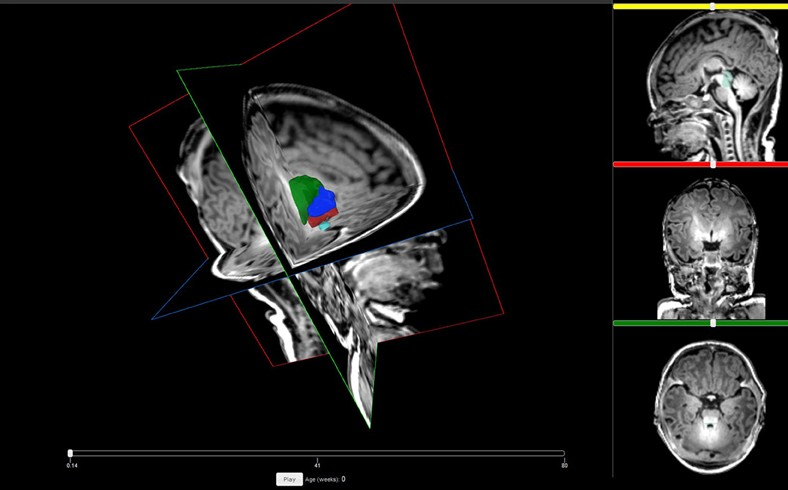
\includegraphics[width=5cm]{plots/05_conv_variations/3d/mri.jpg}
        \caption{Illustration of depth $1$ volumetric data: MRI scan. Each slice of the stack has depth $1$, as the frames are black-white.}
    \end{figure}
\end{vbframe}

\begin{vbframe}{3D Convolutions -- Data}
    \begin{figure}
        \centering
        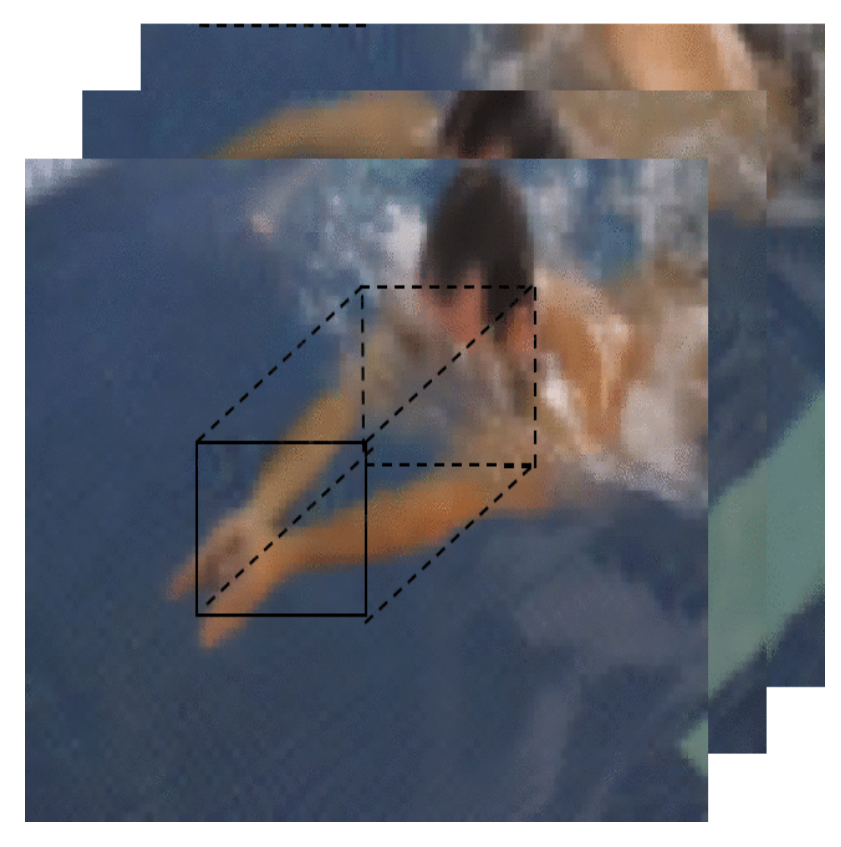
\includegraphics[width=5cm]{plots/05_conv_variations/3d/swim.png}
        \caption{Illustration of volumetric data with depth $> 1$: video snippet of an action detection task. The video consists of several slices, stacked in temporal order. Frames have depth $3$, as they are RGB.}
    \end{figure}
\end{vbframe}
%%%%%%%%%%%%%%%%%%%%%%%%%%%%%%%%%%%%%%%%%%%%%%%%%

\begin{vbframe}{3D Convolutions}
    \begin{figure}
        \centering
        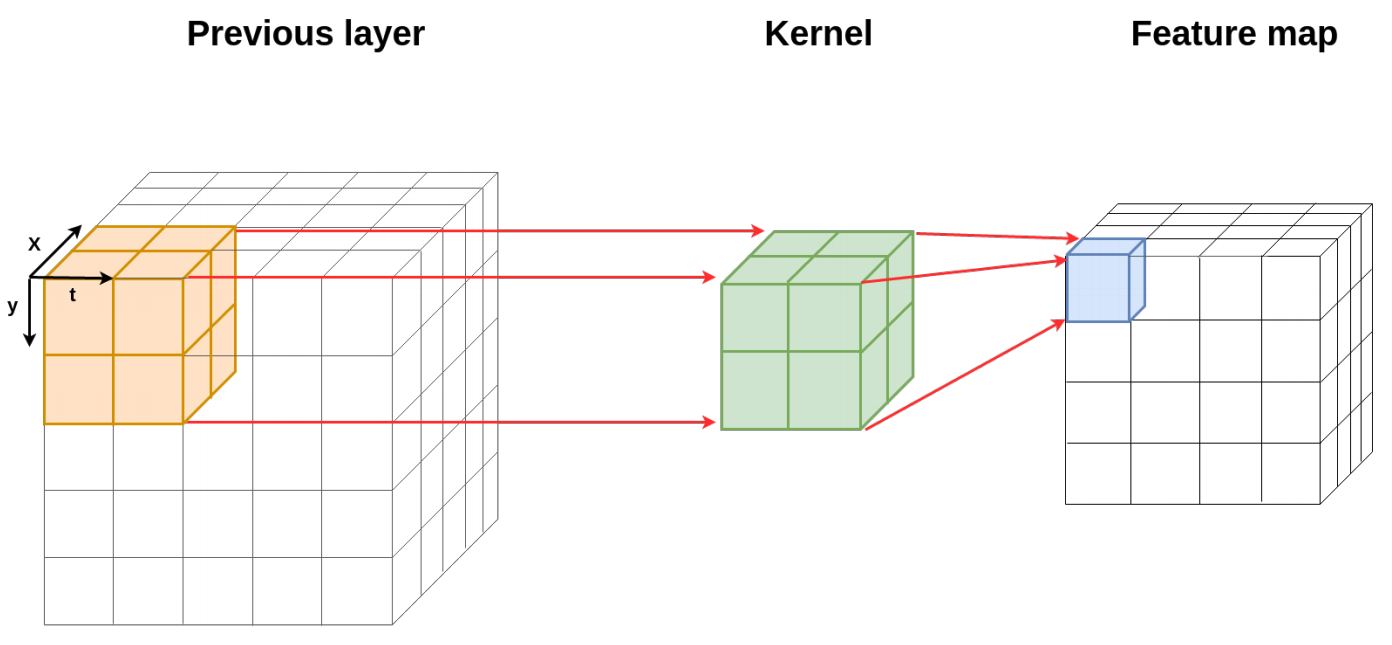
\includegraphics[width=8cm]{plots/05_conv_variations/3d/3dconv.png}
    \end{figure}
    \begin{itemize}
        \item Note: 3D convolutions yield a 3D output.
        % \item 3D convolution can be expressed as: 
        % $$ H(i, j, k) = (\mathcal{I}\star\mathcal{G})(i, j, k)=\sum_{x}\sum_{y}\sum_{z}\mathcal{I}(x, y, z)\mathcal{G}(i-x, j-y, k-z) $$
    \end{itemize}
\end{vbframe}

\begin{vbframe}{3D Convolutions}
    % https://dspace.cc.tut.fi/dpub/bitstream/handle/123456789/24703/teivas.pdf?sequence=1&isAllowed=y
    \begin{figure}
        \centering
        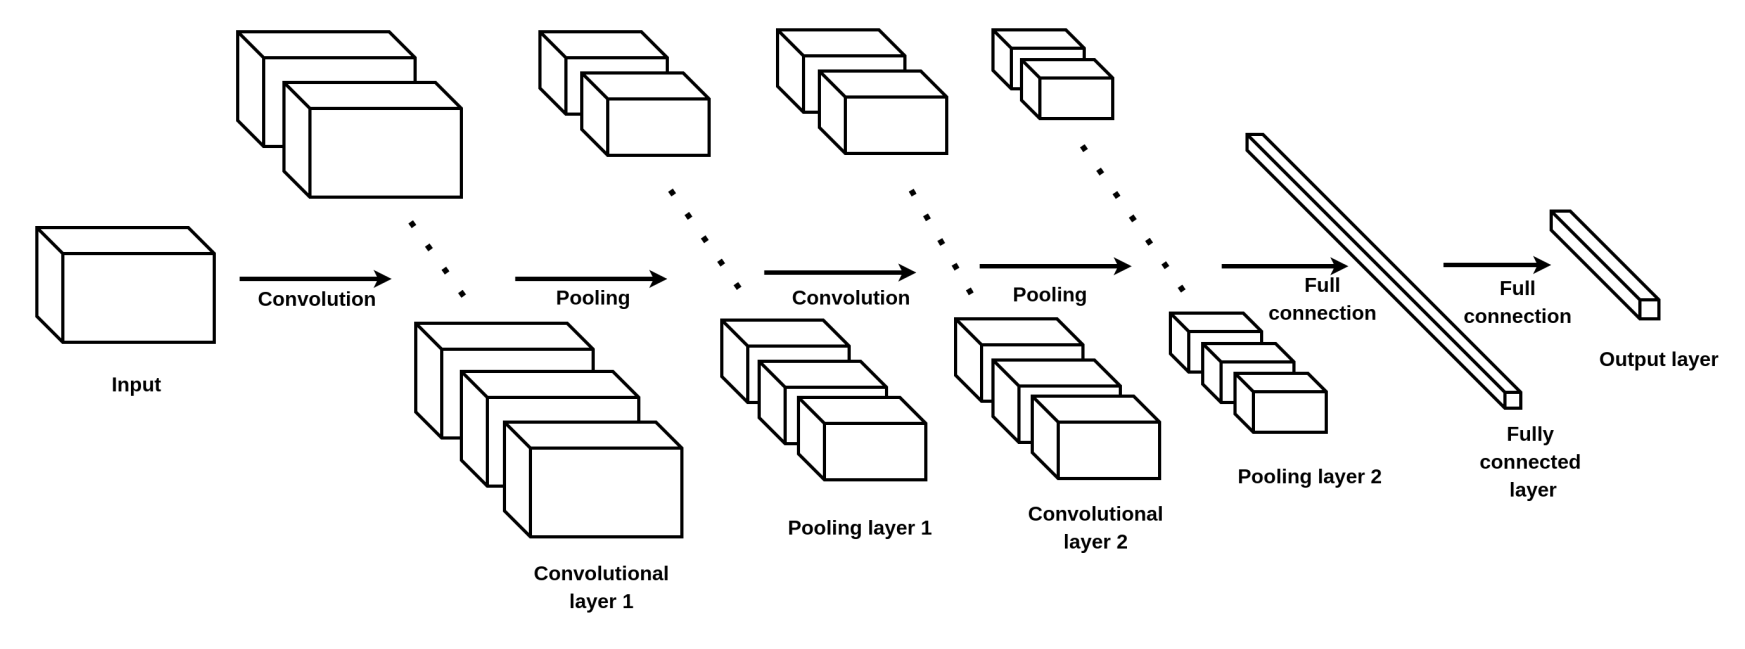
\includegraphics[width=11cm]{plots/05_conv_variations/3d/3dconv_arch.png}
        \caption{Basic 3D-CNN architecture.}
    \end{figure}
    \begin{itemize}
        \item Basic architecture of the CNN stays the same.
        \item 3D convolutions output 3D feature maps which are element-wise activated and then (eventually) pooled in 3 dimensions.
    \end{itemize}
\end{vbframe}
%%%%%%%%%%%%%%%%%%%%%%%%%%%%%%%%%%%%%%%%%%%%%

\section{Dilated Convolutions}

\begin{vbframe}{Dilated convolutions}

    \begin{itemize}
        \item Idea : artificially increase the receptive field of the net without using more filter weights.
        \item The \textbf{receptive field} of a single neuron comprises all inputs that have an impact on this neuron. 
        \item Neurons in the first layers capture less information of the input, while neurons in the last layers have huge receptive fields and can capture a lot more global information from the input. 
        \item The size of the receptive fields depends on the filter size. 
    \end{itemize}

    \vspace*{-0.5cm}

    \begin{figure}
        \centering
        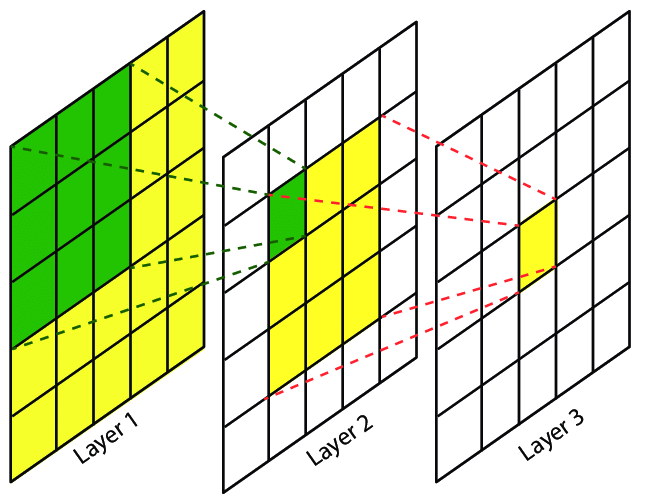
\includegraphics[width=4cm]{plots/05_conv_variations/dilated/receptive_field2.png}
        \caption{Receptive field of each convolution layer with a $3 \times 3$ kernel. The green area marks the receptive field of one pixel in Layer 2, the yellow area marks the receptive field of one pixel in layer 3. } 
    \end{figure}


\begin{itemize}
        \item Intuitively, neurons in the first layers capture less information of the input (layer), while neurons in the last layers have huge receptive fields and can capture a lot more global information from the input (layer). 
        \item The size of the receptive fields depends on the filter size. 
    \end{itemize}

    \vspace*{-0.5cm}

    \begin{figure}
        \centering
        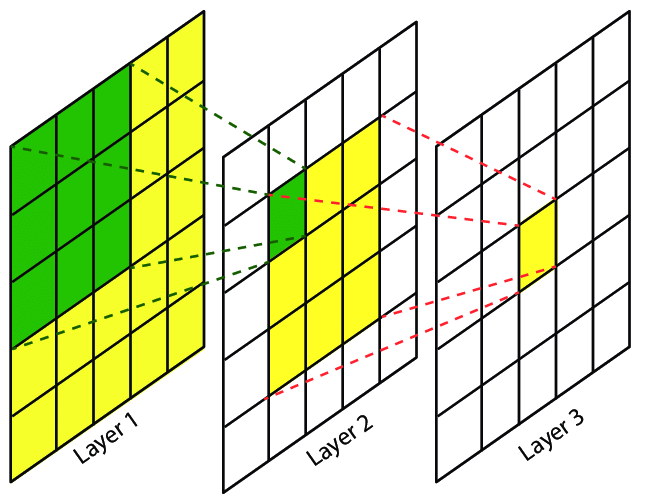
\includegraphics[width=3.5cm]{plots/05_conv_variations/dilated/receptive_field2.png}
        \caption{A convolutional neural network, convolved with $3$ layers with $3 \times 3$ kernels. The green area marks the receptive field of one neuron in Layer 2 w.r.t. the input layer (size $9$), the yellow area marks the receptive field of one pixel in layer 3. } 
    \end{figure}

\framebreak 

\begin{itemize}
        \item By increasing the filter size, the size of the receptive fields increases as well and more contextual information can be captured.
        \item However, increasing the filter size increases the number of parameters, which leads to increased runtime. 
        \item Artificially increase the receptive field of the net without using more filter weights by adding a new dilation parameter to the kernel that skips pixels during convolution.
        \item Benefits:
        \begin{itemize}
            \item Capture more contextual information. 
            \item Enable the processing of inputs in higher dimensions to detect fine details. 
            \item Improved run-time-performance due to less parameters.
        \end{itemize}
    \end{itemize}

    \vspace*{-0.9cm}
 

\framebreak

\begin{itemize}
        \item Useful in applications where the global context is of great importance for the model decision.
        \item This component finds application in:
        \begin{itemize}
            \item Generation of audio-signals and songs within the famous Wavenet developed by DeepMind.
            \item Time series classification and forecasting.
            \item Image segmentation.
        \end{itemize}
    \end{itemize}

    \begin{figure}
        \centering
        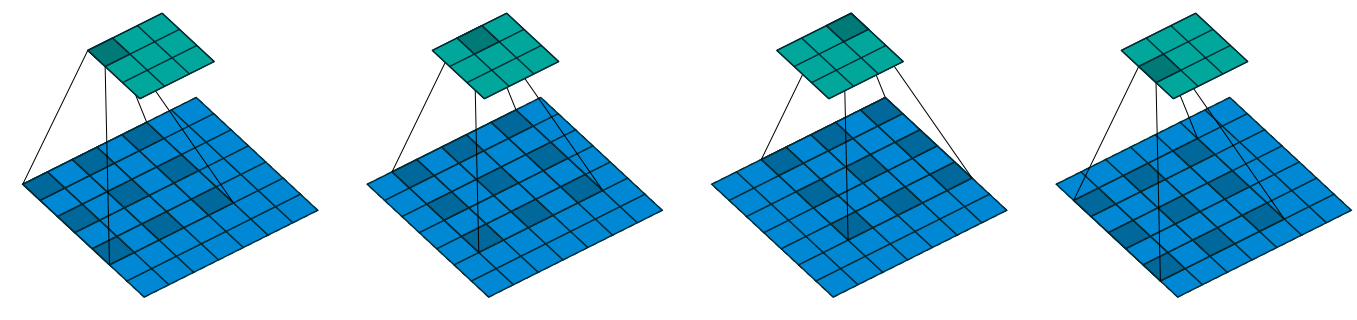
\includegraphics[width=10cm]{plots/05_conv_variations/dilated/dilation_nice.png}
        \caption{Dilated convolution on 2D data. A dilated kernel is a regular convolutional kernel interleaved with zeros. } 
    \end{figure}


\framebreak 

    \vspace*{0.5cm}
    \begin{figure}
        \centering
        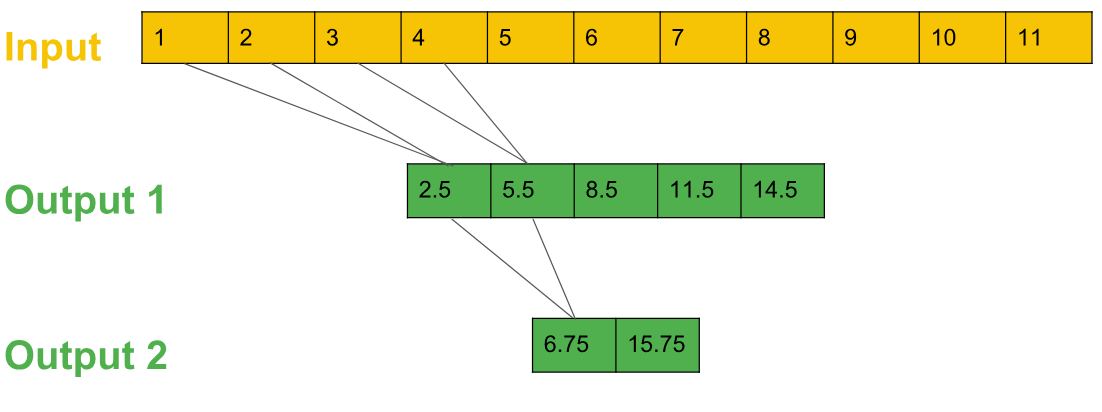
\includegraphics[width=11cm]{plots/05_conv_variations/dilated/classic_conv.png}
        \caption{Simple $1$D convolutional network with convolutional kernel of size $2$, stride $2$ and fixed weights $\{0.5, 1.0\}$. \\ The kernel is not dilated (\textbf{dilation factor} $\mathbf{1}$). One neuron in layer $2$ has a receptive field of size $4$ w.r.t. the input layer. }
    \end{figure}
\framebreak 
    \vspace*{0.5cm}
    \begin{figure}
        \centering
        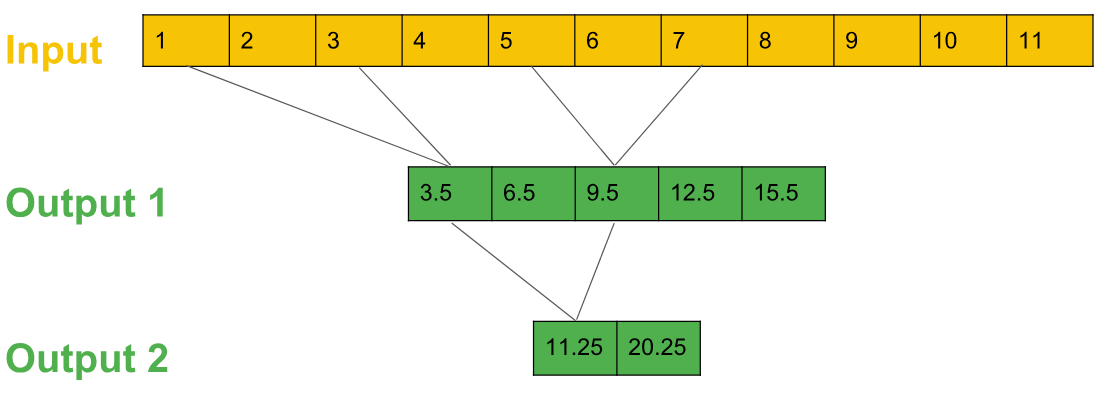
\includegraphics[width=11cm]{plots/05_conv_variations/dilated/dilated.png}
        \caption{Simple $1$D convolutional network with convolutional kernel of size $2$, stride $2$ and fixed weights $\{0.5, 1.0\}$. \\ The kernel is dilated with \textbf{dilation factor} $\mathbf{2}$. One neuron in layer $2$ has a receptive field of size $7$ w.r.t. the input layer. }
    \end{figure}
    
\framebreak 

    \begin{figure}
        \centering
        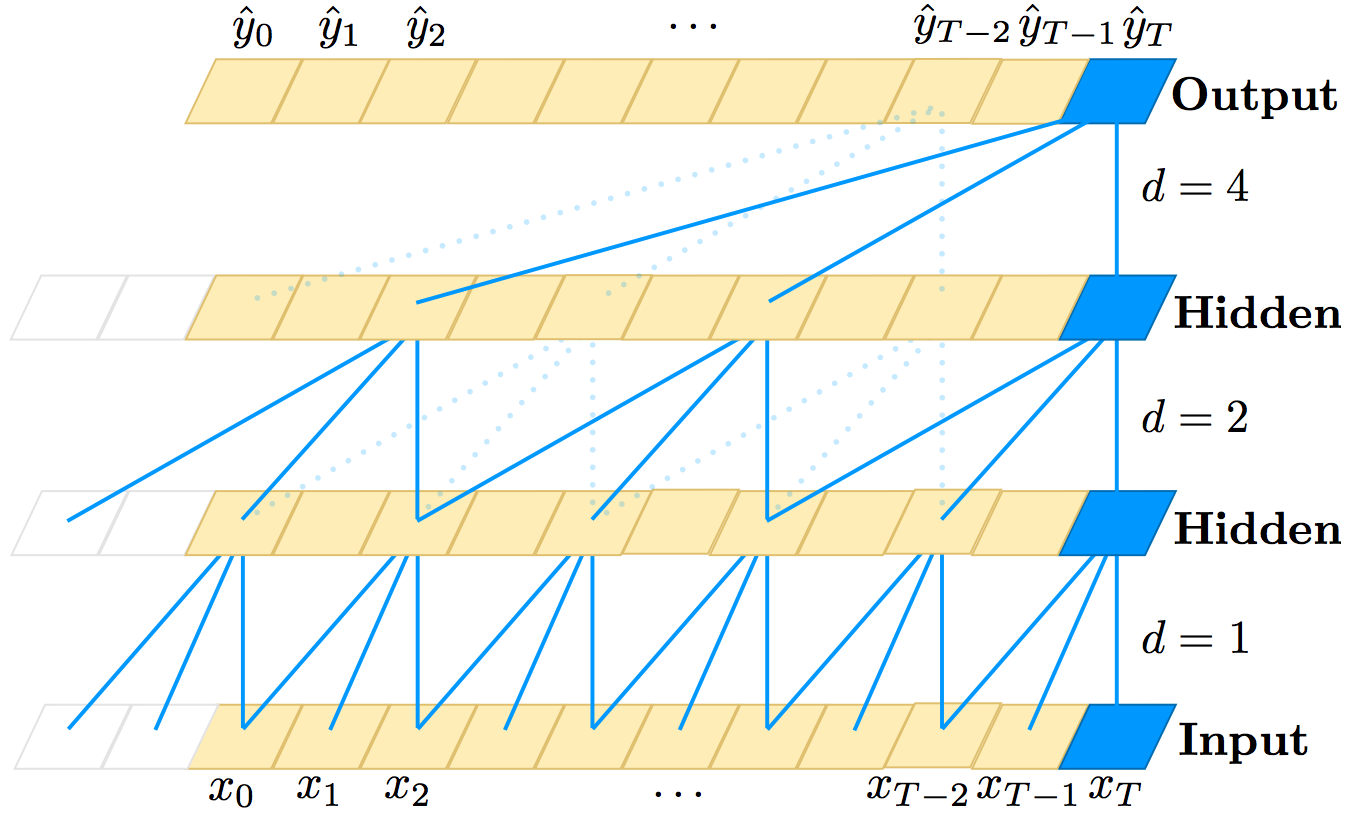
\includegraphics[width=8cm]{plots/05_conv_variations/dilated/tcn.png}
        \caption{Application of (a variant of) dilated convolutions on time series for classification or seq2seq prediction (e.g. machine translation). Given an input sequence $x_0,x_1, \ldots, x_T$, the model generates an output sequence $\yh_0,\yh_1, \ldots, \yh_T$ . Dilation factors $d = 1, 2, 4$ shown above, each with a kernel size $k = 3$. The dilations are used to drastically increase the context information for each output neuron with relatively few layers.}
    \end{figure}

\end{vbframe}
%%%%%%%%%%%%%%%%%%%%%%%%%%%%%%%%%%%%%%%%%%%%

\section{Transposed Convolutions}


\begin{vbframe}{Transposed convolutions}
    \begin{itemize}
        \item Problem setting: 
        \begin{itemize}
            \item For many applications and in many network architectures, we often want to do transformations going in the opposite direction of a normal convolution, i.e. we would like to perform up-sampling.
            \item examples include generating high-resolution images and mapping low dimensional feature map to high dimensional space such as in auto-encoder or semantic segmentation.
        \end{itemize}
        \item Instead of decreasing dimensionality as with regular convolutions, \textbf{transposed convolutions} are used to re-increase dimensionality back to the initial dimensionality.
        %\item Idea: use transposed convolutions to re-increase dimensionality instead of decreasing it as with regular convolutions.
        \item Note: Do not confuse this with deconvolutions (which are mathematically defined as the inverse of a convolution).
    \end{itemize}
    
\framebreak

\begin{itemize}
\item Example 1:
  \begin{itemize}
  \item Input: blue feature map with dim $4\times 4$.
  \item Output: turquoise feature map with dim $2\times 2$.
  \end{itemize}
\end{itemize}
\begin{figure}
\centering
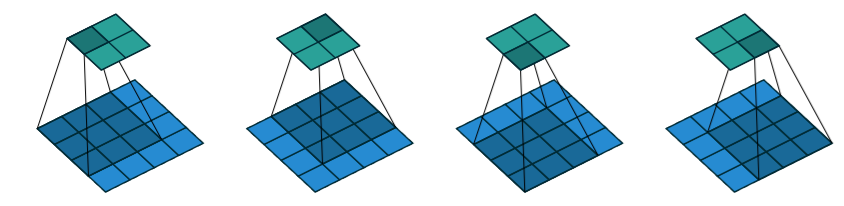
\includegraphics[width=10cm]{plots/05_conv_variations/transpose/transpose_conv_0.png}
      \caption{ A \textbf{regular} convolution with kernel-size $k$ = 3, padding $p$ = 0 and stride $s$ = 1.}
\end{figure}
    Here, the feature map shrinks from $4\times 4$ to $2\times 2$.

\framebreak

\begin{itemize}
\item Example 1:
        \small{
        \begin{itemize}
        \item Now, let us upsample the $2\times 2$ feature map back to a $4\times 4$ feature map.
        \item Input: $2\times 2$ (blue). Output: $4\times 4$ (turquoise).
        \end{itemize}
\item One way to upsample is to use a regular convolution with various padding strategies.}
\end{itemize}
\begin{figure}
\centering
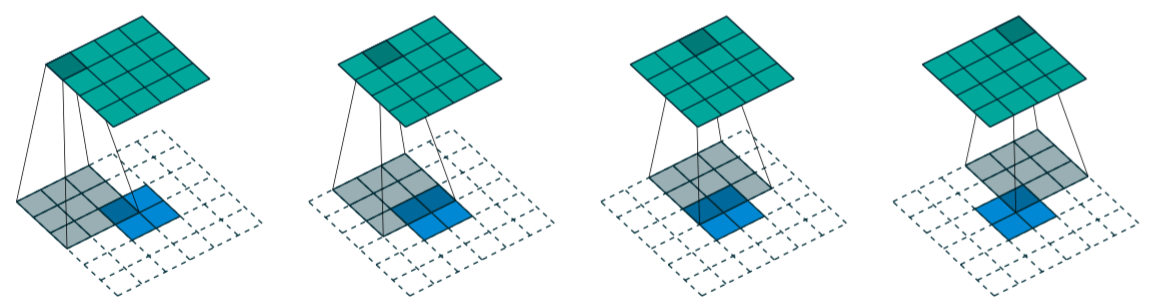
\includegraphics[width=10cm]{plots/05_conv_variations/transpose/transpose_conv.png}
\caption{\textbf{Transposed} convolution can be a seen as a regular convolution. Convolution (above) with $k' = 3, s' = 1, p' = 2$ re-increases dimensionality from $2\times 2$ to $4\times 4$}
\end{figure}
    
\framebreak

\begin{itemize}
\item Convolution with parameters kernel size $k$, stride $s$ and padding factor $p$
\item Associated transposed convolution has parameters $k' = k$, $s' = s$ and $p' = k-1$
\end{itemize}

\framebreak
Example 2 : Convolution as a matrix multiplication : 
% \framebreak
%   Example 2 : Let's now view transposed convolutions from a different perspective.
\begin{figure}
\centering
\scalebox{0.75}{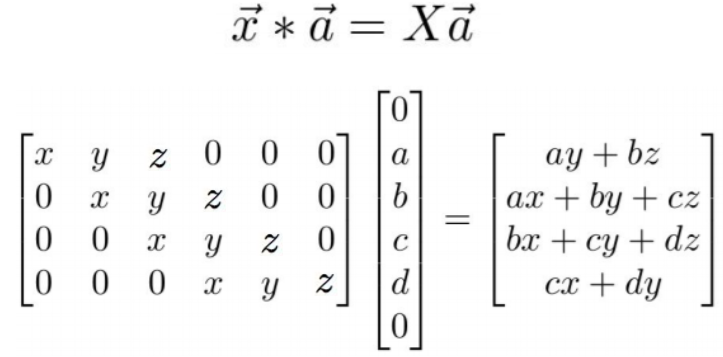
\includegraphics{plots/05_conv_variations/transpose/transpose_mat_1.png}}
\tiny{\\credit:Stanford University}
\caption{A "regular" 1D convolution. stride = 1 , padding = 1. The vector $a$ is the 1D input feature map. }
\end{figure}
   
  
\framebreak
Example 2 : Transposed Convolution as a matrix multiplication :
\begin{figure}
\centering
\scalebox{0.6}{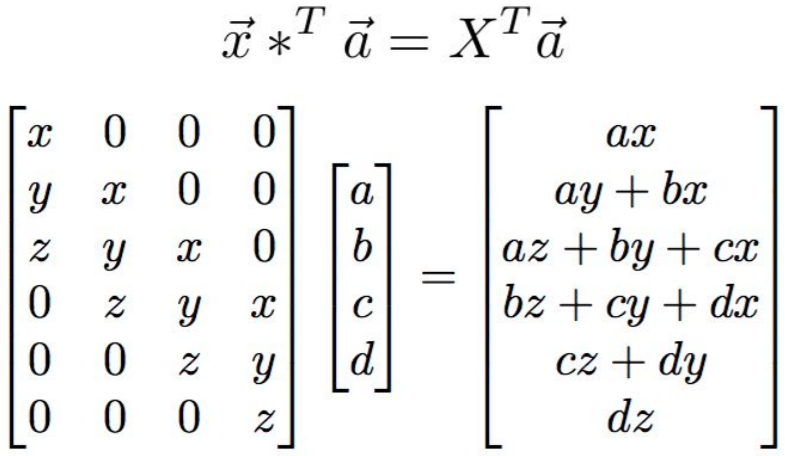
\includegraphics{plots/05_conv_variations/transpose/transpose_mat_2.png}}
\tiny{\\credit:Stanford University}
\caption{"Transposed" convolution upsamples a vector of length 4 to a vector of length 6. Stride is 1. Note the change in padding.}
\end{figure}
\small{Important : Even though the "structure" of the matrix here is the transpose of the original matrix, the non-zero elements are, in general, different from the correponding elements in the original matrix. These (non-zero) elements/weights are tuned by backpropagation.} 

\framebreak 

Example 3: Transposed Convolution as matrix multiplication:
\begin{figure}
\centering
\scalebox{0.85}{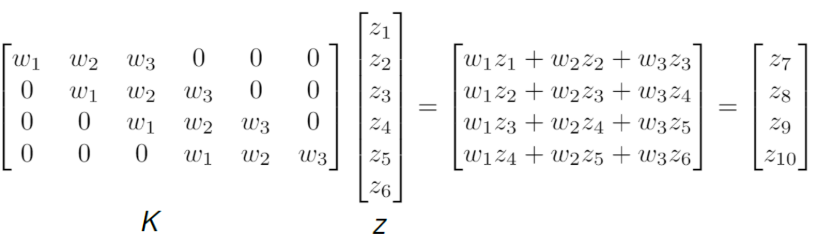
\includegraphics{plots/05_conv_variations/transpose/tr_ex21.png}}
\caption{A regular 1D convolution with  stride = 1 ,and padding = 0. The vector $z$ is in the input feature map. The matrix $K$ represents the convolution operation.}
\end{figure}
  A regular convolution decreases the dimensionality of the feature map from 6 to 4.\\
\end{vbframe}
%%%%%%%%%%%%%%%%%%%%%%%%%%%%%%%%%%%%%%%%%%%%

\begin{frame}{Transposed Convolutions}

Example 3: Transposed Convolution as matrix multiplication:
\vspace*{-0.2cm}
\begin{figure}
\centering
\scalebox{0.75}{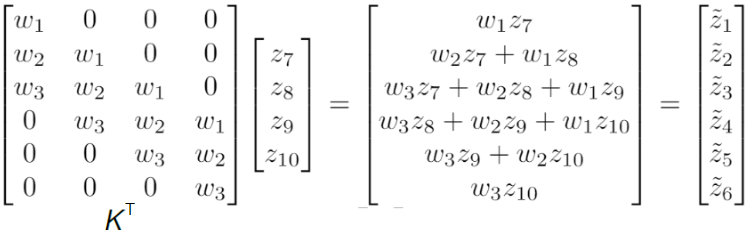
\includegraphics{plots/05_conv_variations/transpose/tr_ex22.png}}
\caption{\footnotesize{A transposed convolution can be used to upsample the feature vector of length 4 back to a feature vector of length 6.}}
\end{figure}

\vspace*{-0.4cm}

\textbf{Note}:
\begin{itemize}
  	\only<1>{\item Even though the transpose of the original matrix is shown in this example, the actual values of the weights are different from the original matrix (and optimized by backpropagation). }
  	\only<1>{\item The goal of the transposed convolution here is simply to get back the original dimensionality. It is \textit{not} necessarily to get back the original feature map itself.}
  	\only<2>{\item The elements in the downsampled vector only affect those elements in the upsampled vector that they were originally "derived" from. For example, $z_7$ was computed using $z_1$ , $z_2$ and $z_3$ and it is only used to compute $\tilde{z}_1$, $\tilde{z}_2$ and $\tilde{z}_3$.}
  	\only<2>{\item In general, transposing the original matrix does not result in a convolution. But a transposed convolution can always be implemented as a regular convolution by using various padding strategies (this would not be very efficient, however).}
\end{itemize}

\end{frame}
%%%%%%%%%%%%%%%%%%%%%%%%%%%%%%%%%%%%%%%%%%%

\begin{frame}{Transposed Convolutions}
  
  Example 4: Let us now view transposed convolutions from a different perspective.
  
  \only<1>{
  \begin{figure}
      \centering
      \scalebox{0.9}{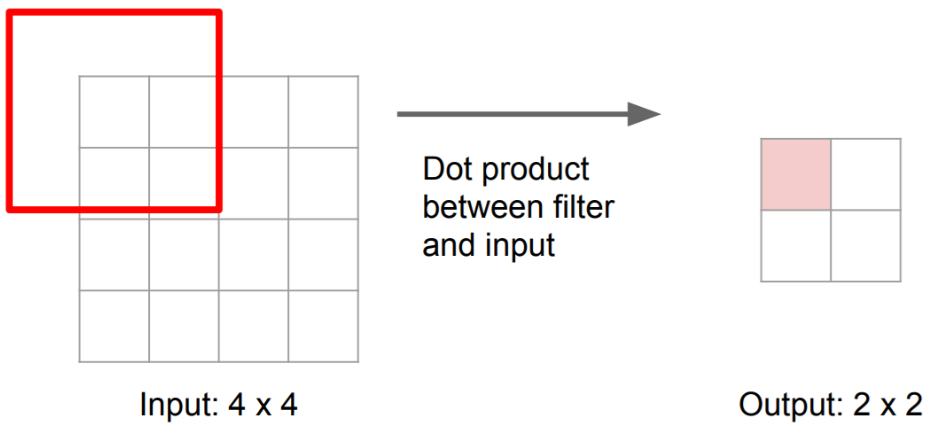
\includegraphics{plots/05_conv_variations/transpose/tr_conv_1.png}}
      \tiny{\\credit: Stanford University}
      \caption{Regular $3\times 3$ convolution, stride 2, padding 1.}
  \end{figure}
 }

  \only<2>{
  \begin{figure}
      \centering
      \scalebox{0.9}{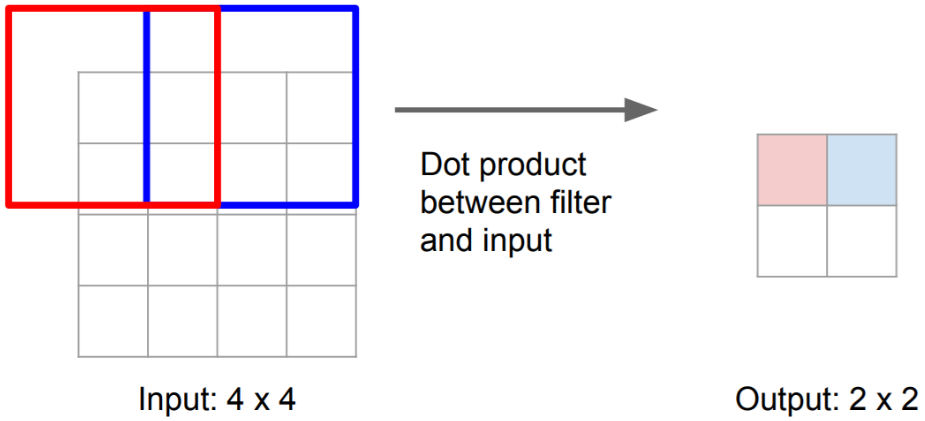
\includegraphics{plots/05_conv_variations/transpose/tr_conv_2.png}}
      \tiny{\\credit: Stanford University}
      \caption{Regular $3\times 3$ convolution, stride 2, padding 1.}
  \end{figure}
 }

  \only<3>{
  \begin{figure}
      \centering
      \scalebox{0.8}{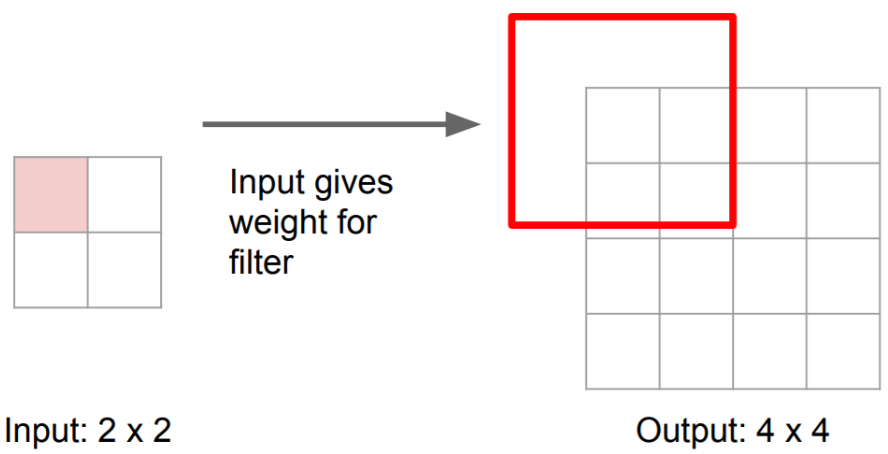
\includegraphics{plots/05_conv_variations/transpose/tr_conv_3.png}}
      \tiny{\\credit: Stanford University}
      \caption{\textit{Transposed} $3\times 3$ convolution, stride 2, padding 1. Note: stride now refers to the "stride" in the \textit{output}.}
  \end{figure}

   Here, the filter is \textit{scaled} by the input.\\

 }

  \only<4>{
  \begin{figure}
      \centering
      \scalebox{0.8}{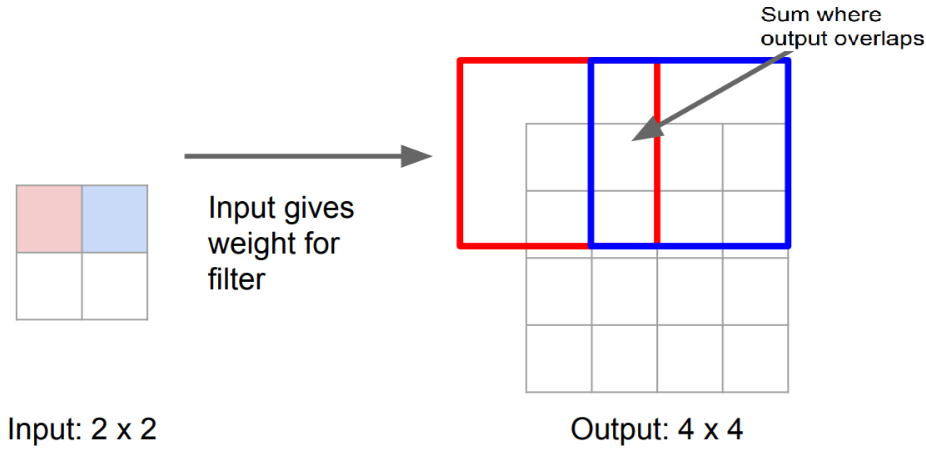
\includegraphics{plots/05_conv_variations/transpose/tr_conv_4.png}}
      \tiny{\\credit: Stanford University}
      \caption{\textit{Transposed} $3\times 3$ convolution, stride 2, padding 1. Note: stride now refers to the "stride" in the \textit{output}.}
  \end{figure}
  Here, the filter is \textit{scaled} by the input.

 }

\end{frame}
%%%%%%%%%%%%%%%%%%%%%%%%%%%%%%%%%%%%%%

\begin{vbframe}{Transposed Convolutions -- drawback}
    \begin{figure}
        \centering
        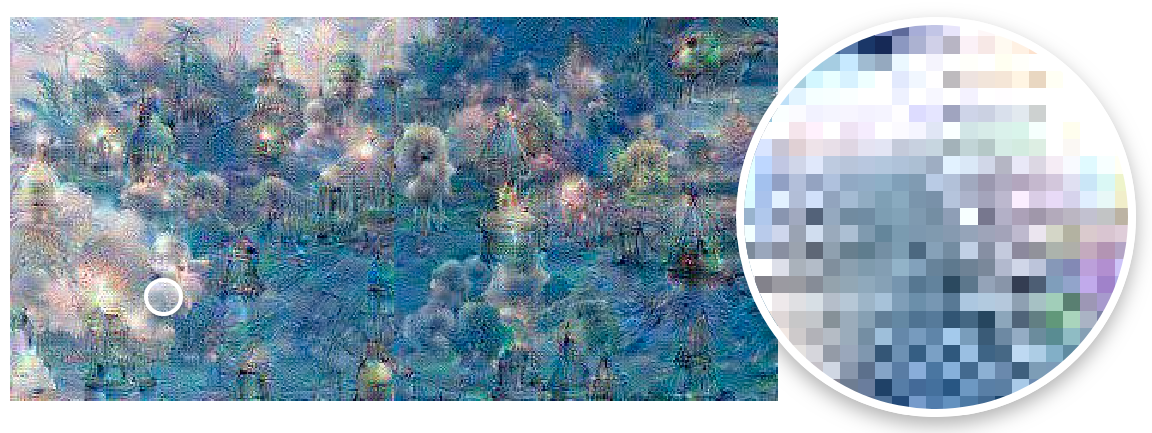
\includegraphics[width=8cm]{plots/05_conv_variations/transpose/transpose_artifact.png}
        \caption{Artifacts produced by transposed convolutions.}
    \end{figure}
    \begin{itemize}
        \item Transposed convolutions lead to checkerboard-style artifacts in resulting images.
    \end{itemize}
    
\framebreak

\begin{itemize}
        \small{\item Explanation: transposed convolution yields an overlap in some feature map values.
        \item This leads to higher magnitude for some feature map elements than for others, resulting in the checkerboard pattern.
        \item One solution is to ensure that the kernel size is divisible by the stride.
        }
    \end{itemize}
        \begin{figure}
            \centering
              \scalebox{0.65}{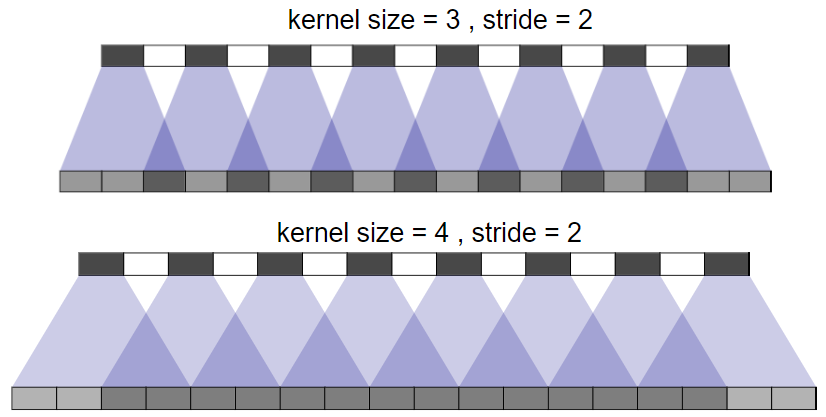
\includegraphics{plots/05_conv_variations/transpose/deconv_blog.png}}
            \caption{\footnotesize{1D example. In both images, top row = input and bottom row = output. \textit{Top}: Here, kernel weights overlap unevenly which results in a checkerboard pattern. \textit{Bottom}: There is no checkerboard pattern as the kernel size is divisible by the stride.}}
        \end{figure}
       
\framebreak

\begin{itemize}
         \item Solutions: 
         \begin{itemize}
             \item Increase dimensionality via upsampling (bilinear, nearest neighbor) and then convolve this output with regular convolution.
             \item Make sure that the kernel size $k$ is divisible by the stride $s$.
         \end{itemize}
     \end{itemize}
     \begin{figure}
         \centering
         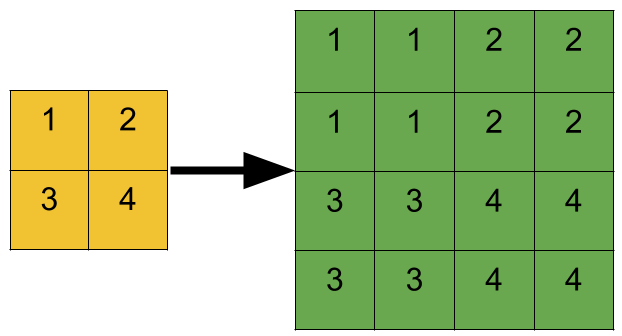
\includegraphics[width=5cm]{plots/05_conv_variations/transpose/upsample.png}
         \caption{Nearest neighbor upsampling and subsequent same convolution to avoid checkerboard patterns.}
     \end{figure}
\end{vbframe}
%%%%%%%%%%%%%%%%%%%%%%%%%%%%%%%%%%%%%%%%%%%

\section{Separable Convolutions}

 \begin{vbframe}{Separable convolutions}
     \begin{itemize}
         \item Separable Convolutions are used in some neural net architectures, such as the MobileNet.
         \item Motivation: make convolution computationally more efficient.
         \item One can perform:
               \begin{itemize}
                   \item spatially separable convolution 
                   \item depthwise separable convolution.
                \end{itemize}
      \end{itemize}
      \textbf{spatially separable convolution}: The spatially separable convolution operates on the 2D spatial dimensions of images, i.e. height and width. Conceptually, spatially separable convolution decomposes a convolution into two separate operations.
      \begin{itemize}   
         \item Consider the sobel kernel from the previous lecture:
             \begin{equation*}
                     G_x = 
                     \begin{bmatrix}
                         +1 & 0 & -1 \\
                         +2 & 0 & -2 \\
                         +1 & 0 & -1 
                     \end{bmatrix}
             \end{equation*}
         \item this 3x3 dimensional kernel can be replaced by the outer product of two 3x1 and 1x3 dimensional kernels:
            \begin{equation*}
                     \begin{bmatrix}
                         +1 \\ 
                         +2 \\
                         +1   
                     \end{bmatrix}* 
                     \begin{bmatrix}
                         +1 & 0 & -1   
                     \end{bmatrix}
             \end{equation*}
         \item Convolving with both filters subsequently has a similar effect, reduces the amount of parameters to be stored and thus improves speed:
              \begin{figure}
         \centering
         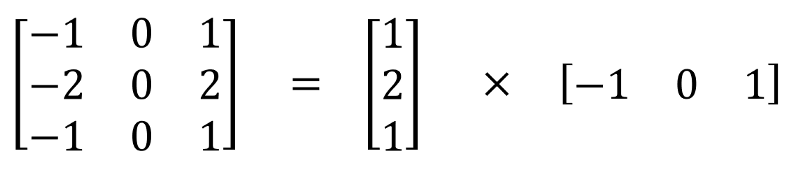
\includegraphics[width=6cm]{plots/05_conv_variations/separable/seprablematrix.png}
         \caption{In convolution, the 3x3 kernel directly convolves with the image. In spatially separable convolution, the 3x1 kernel first convolves with the image. Then the 1x3 kernel is applied. This would require 6 instead of 9 parameters while doing the same operations.}
     \end{figure}
     \end{itemize}
 \end{vbframe}
%%%%%%%%%%%%%%%%%%%%%%%%%%%%%%%%%%%%%%%%

\begin{vbframe}{Spatially separable convolution}
  
  Example 1: A convolution on a $5 \times 5$ image with a $3 \times 3$ kernel (stride=1, padding=0) requires scanning the kernel at 3 positions horizontally and 3 vertically. That is 9 positions in total, indicated as the dots in the image below. At each position, 9 element-wise multiplications are applied. Overall, that is 9 x 9 = 81 multiplications.
     \begin{figure}
         \centering
         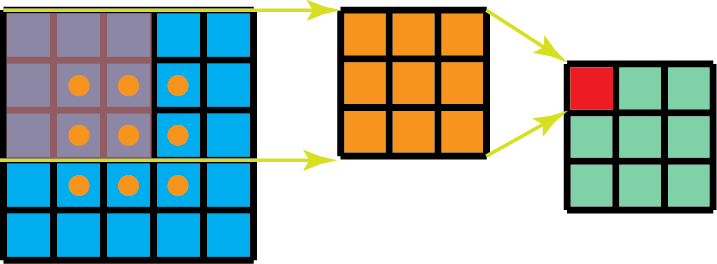
\includegraphics[width=4cm]{plots/05_conv_variations/separable/sep0.png}
         \caption{Standard convolution with 1 channel.}
     \end{figure}
   
     \begin{figure}
         \centering
         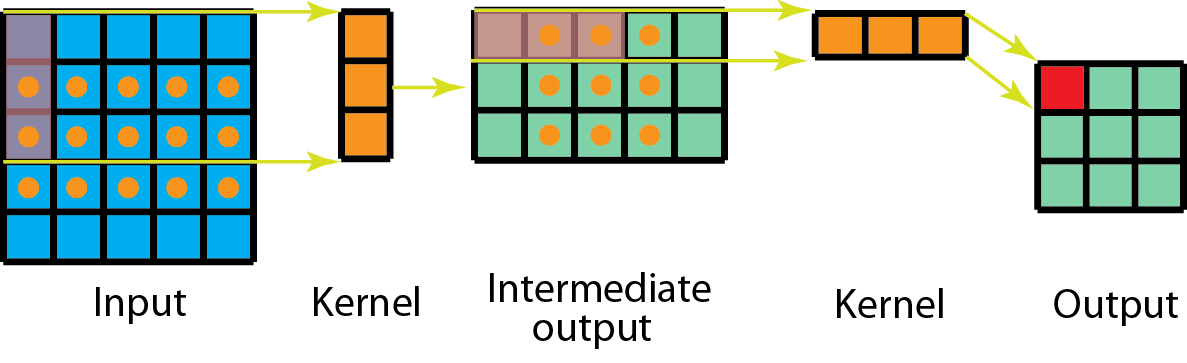
\includegraphics[width=8cm]{plots/05_conv_variations/separable/sep1.png}
         \caption{Spatially separable convolution with 1 channel. Overall, the spatially separable convolution takes 45 + 27 = 72 multiplications. (Image source: Bai (2019))}
     \end{figure}
     
    

   \textbf{Note:} However, despite their advantages, spatial separable convolutions are seldom applied in deep learning. This is mainly due to not all kernels being able to get divided into two smaller ones. Replacing all standard convolutions by spatial separable would also introduce a limit in searching for all possible kernels in the training process, implying worse training results.
   
\end{vbframe}
%%%%%%%%%%%%%%%%%%%%%%%%%%%%%%%%%%%%%%%%

\begin{vbframe}{Depthwise separable convolution}
   \begin{itemize}
     \item The depthwise separable convolutions, which is much more commonly used in deep learning (e.g. in MobileNet and Xception).
     \item This convolution separates convolutional process into two stages of depthwise and pointwise.
   \end{itemize}

 
\begin{figure}
\centering
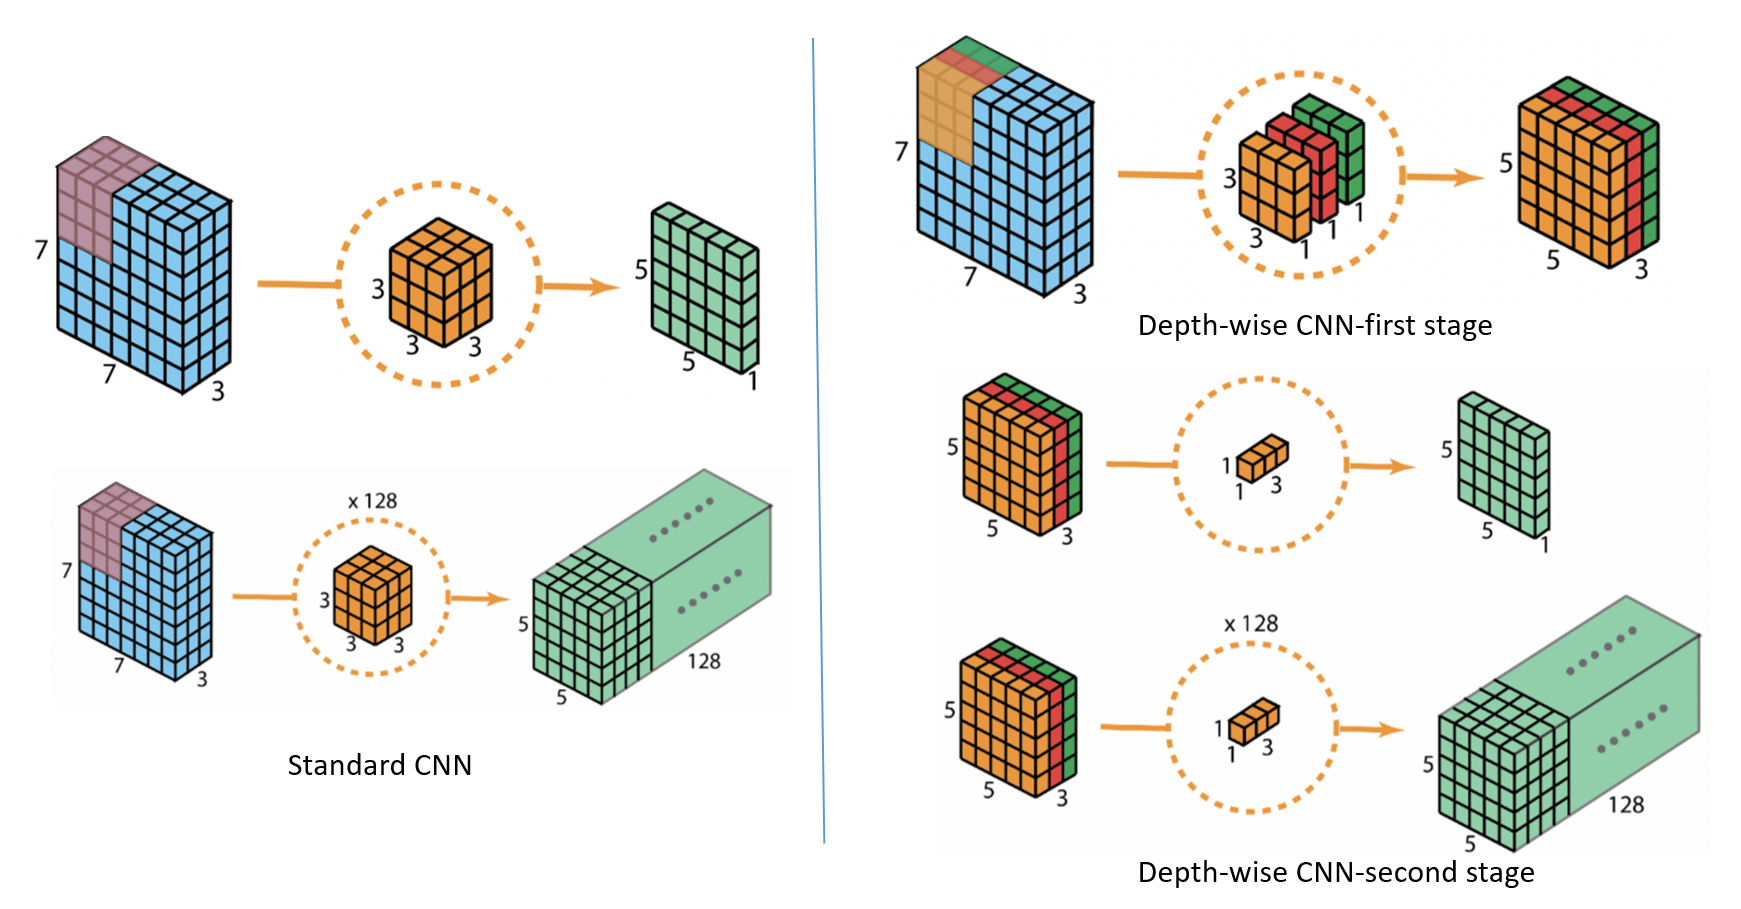
\includegraphics[width=8cm]{plots/05_conv_variations/separable/Depthwise.png}
\caption{Comparision between standard cnn and separable depthwise cnn}
\end{figure}
     
     
\begin{figure}
\centering
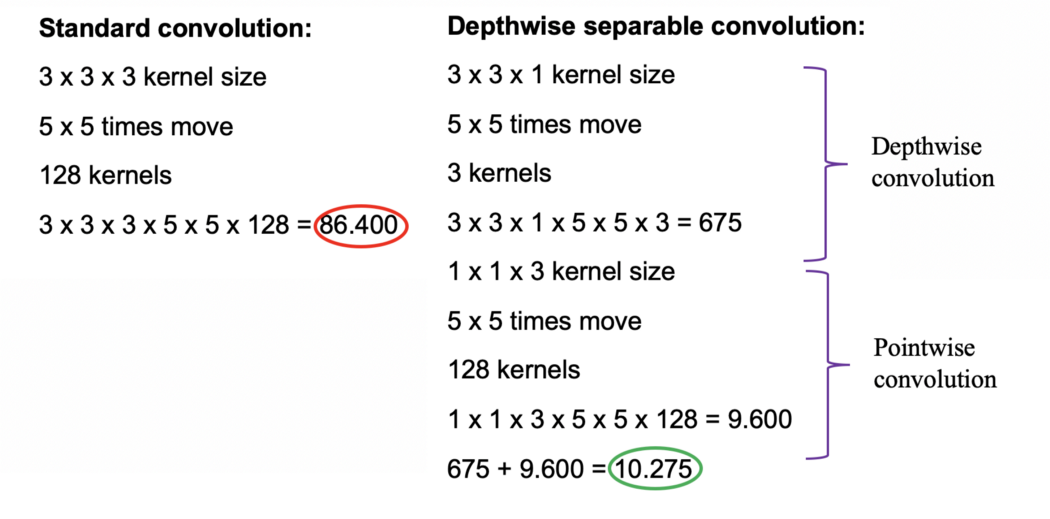
\includegraphics[width=10cm]{plots/05_conv_variations/separable/example-depthwise2.png}
\caption{Comparision of number of multiplications in Depthwise separable cnn and standard cnn}
\end{figure}
     
Therefore, fewer computations leads faster network.
     
\begin{figure}
\centering
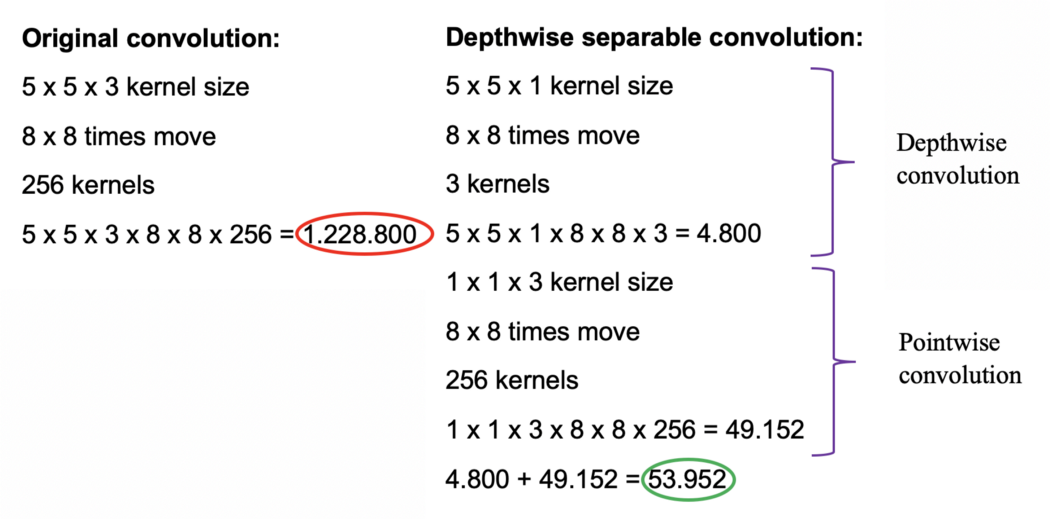
\includegraphics[width=9cm]{plots/05_conv_variations/separable/example-depthwise1.png}
\caption{Comparision of number of multiplications in Depthwise separable cnn and standard cnn}
\end{figure}
     
\end{vbframe}
%%%%%%%%%%%%%%%%%%%%%%%%%%%%%%%%%%%%%%%%

\begin{vbframe}{Depthwise convolution }
 
 As the name suggests, we perform kernel on depth of the input volume (on the input channels). The steps followed in this convolution are:

   \begin{itemize}
     \item Take number of kernels equal to the number of input channels, each kernel having depth 1. Example, if we have a kernel of size $3\times 3$ and an input of size $6\times 6$ with 16 channels, then there will be $16 \times 3 \times 3$ kernels.
     \item Every channel thus has 1 kernel associated with it. This kernel is convolved over the associated channel separately resulting in 16 feature maps.
     \item Stack all these feature maps to get the output volume with $4 \times 4$ output size and 16 channels.
   \end{itemize}

     
\end{vbframe}
%%%%%%%%%%%%%%%%%%%%%%%%%%%%%%%%%%%%%%%

\begin{vbframe}{Pointwise convolution }
 
As the name suggests, this type of convolution is applied to every single point in the convolution separately (remember $1\times 1$ convs?). So how does this work?

   \begin{itemize}
     \item Take a $1\times 1$ conv with number of filters equal to number of channels you want as output.
     \item Perform basic convolution applied in $1\times 1$ conv to the output of the Depth-wise convolution.
   \end{itemize}

     
\end{vbframe}
%%%%%%%%%%%%%%%%%%%%%%%%%%%%%%%%%%%%%%%%%

\section{Flattened Convolutions}

\begin{vbframe}{Flattened Convolution}
    
Flattening is converting the data into a 1-dimensional array for inputting it to the next layer. We flatten the output of the convolutional layers to create a single long feature vector. And it is connected to the final classification model, which is called a fully-connected layer.
          
\begin{figure}
\centering
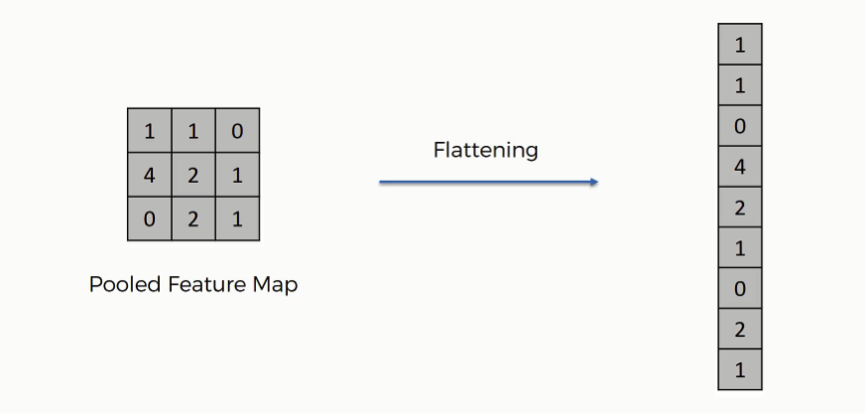
\includegraphics[width=5cm]{plots/05_conv_variations/flaten/flat1.png}
\end{figure}
     
\begin{figure}
\centering
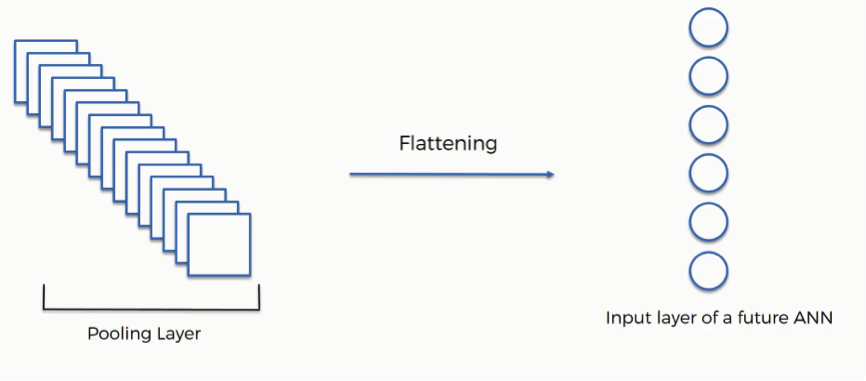
\includegraphics[width=5cm]{plots/05_conv_variations/flaten/flat2.png}
\end{figure}

\end{vbframe}



%%%%%%%%%%%%%%%%%%%%%%%%%%%%%%%%%%%%%%%%%%%%%%%%%%%%%%%%%%%%%%%%%%
%%%%%%%%%%%%%%%%%%%%%%%%%%%%%%%%%%%%%%%%%%%%%%%%%%%%%%%%%%%%%%%%%%
%%%%%%%%%%%%%%%%%%          REFERENCES          %%%%%%%%%%%%%%%%%%
%%%%%%%%%%%%%%%%%%%%%%%%%%%%%%%%%%%%%%%%%%%%%%%%%%%%%%%%%%%%%%%%%%
\begin{vbframe}
\frametitle{References}
\footnotesize{
\begin{thebibliography}{99}

\bibitem[Dumoulin et al., 2016]{14} Dumoulin, Vincent and Visin, Francesco (2016)
\newblock A guide to convolution arithmetic for deep learning
\newblock \emph{\url{https://arxiv.org/abs/1603.07285v1}}
%%%%%%%%%%%%%%%%%%%%%%%%%%%%%%%%%%
\bibitem[van den Oord et al., 2016]{15} Van den Oord, Aaron, Sander Dielman, Karen Simonyan, Oriol Vinyals, Alex Graves, Nal Kalchbrenner, and Koray Kavukocuoglu (2016)
\newblock WaveNet: A Generative Model for Raw Audio
\newblock \emph{\url{https://arxiv.org/abs/1609.03499}}
%%%%%%%%%%%%%%%%%%%%%%%%%%%%%%%%%%
%%%%%%%%%%%%%%%%%%%%%%%%%%%%%%%%%%
\bibitem[Gennart et al., 1996]{17} Benoit A., Gennart, Bernard Krummenacher, Roger D. Hersch, Bernard Saugy, J.C. Hadorn and D. Mueller (1996)
\newblock The Giga View Multiprocessor Multidisk Image Server
\newblock \emph{\url{https://www.researchgate.net/publication/220060811_The_Giga_View_Multiprocessor_Multidisk_Image_Server}}
%%%%%%%%%%%%%%%%%%%%%%%%%%%%%%%%%%
%%%%%%%%%%%%%%%%%%%%%%%%%%%%%%%%%%
\bibitem[Tran et al., 2015]{18} Tran, Du, Lubomir Bourdev, Rob Fergus,  Lorenzo Torresani and Paluri Manohar (2015)
\newblock Learning Spatiotemporal Features with 3D Convolutional Networks
\newblock \emph{\url{https://arxiv.org/pdf/1412.0767.pdf}}
%%%%%%%%%%%%%%%%%%%%%%%%%%%%%%%%%%
%%%%%%%%%%%%%%%%%%%%%%%%%%%%%%%%%%
\bibitem[Milletari et al., 2016]{19} Milletari, Fausto, Nassir Navab and  Seyed-Ahmad Ahmadi (2016)
\newblock V-Net: Fully Convolutional Neural Networks for
Volumetric Medical Image Segmentation
\newblock \emph{\url{https://arxiv.org/pdf/1606.04797.pdf}}
%%%%%%%%%%%%%%%%%%%%%%%%%%%%%%%%%%
%%%%%%%%%%%%%%%%%%%%%%%%%%%%%%%%%%
\bibitem[Zhang et al., 2015]{20} Zhang, Xiang, Junbo Zhao and Yann LeCun (2015)
\newblock Character-level Convolutional Networks for Text Classification
\newblock \emph{\url{http://arxiv.org/abs/1509.01626}}
%%%%%%%%%%%%%%%%%%%%%%%%%%%%%%%%%%
%%%%%%%%%%%%%%%%%%%%%%%%%%%%%%%%%%
\bibitem[Wang et al., 2017]{21} Wang, Zhiguang, Weizhong Yan and Tim Oates (2017)
\newblock Time Series Classification from Scratch with Deep Neural Networks: A Strong Baseline
\newblock \emph{\url{http://arxiv.org/abs/1509.01626}}
%%%%%%%%%%%%%%%%%%%%%%%%%%%%%%%%%%
%%%%%%%%%%%%%%%%%%%%%%%%%%%%%%%%%%
\bibitem[Yu et. al, 2015]{22} Fisher Yu and Vladlen Koltun (2015)
\newblock Multi-Scale Context Aggregation by Dilated Convolutions
\newblock \emph{\url{https://arxiv.org/abs/1511.07122}}
%%%%%%%%%%%%%%%%%%%%%%%%%%%%%%%%%%
%%%%%%%%%%%%%%%%%%%%%%%%%%%%%%%%%%
\bibitem[Bai et. al, 2018]{23} Bai, Shaojie,  Zico J. Kolter and Vladlen Koltun (2018)
\newblock An Empirical Evaluation of Generic Convolutional and Recurrent Networks for Sequence Modeling
\newblock \emph{\url{http://arxiv.org/abs/1509.01626}}
%%%%%%%%%%%%%%%%%%%%%%%%%%%%%%%%%%
%%%%%%%%%%%%%%%%%%%%%%%%%%%%%%%%%%
\bibitem[Odena et. al , 2017]{24} Augustus Odena, Vincent Dumoulin and Chris Olah (2016)
\newblock Deconvolution and Checkerboard Artifacts
\newblock \emph{\url{https://distill.pub/2016/deconv-checkerboard/}{https://distill.pub/2016/deconv-checkerboard/}}
%%%%%%%%%%%%%%%%%%%%%%%%%%%%%%%%%%
%%%%%%%%%%%%%%%%%%%%%%%%%%%%%%%%%%
\bibitem[Arauho et. al , 2019]{45} Andre Araujo, Wade Norris and Jack Sim (2019)
\newblock Computing Receptive Fields of Convolutional Neural Networks
\newblock \emph{\url{https://distill.pub/2019/computing-receptive-fields/}}
%%%%%%%%%%%%%%%%%%%%%%%%%%%%%%%%%%
%%%%%%%%%%%%%%%%%%%%%%%%%%%%%%%%%%
\bibitem[Wang et. al , 2017]{31} Zhiguang Wang, Yan, Weizhong and Tim Oates (2017)
\newblock Time series classification from scratch with deep neural networks: A
strong baseline
\newblock \emph{\url{https://arxiv.org/1611.06455}}
%%%%%%%%%%%%%%%%%%%%%%%%%%%%%%%%%%
%%%%%%%%%%%%%%%%%%%%%%%%%%%%%%%%%%
\bibitem[Lin et al., 2017]{38} Lin, Haoning and Shi, Zhenwei and Zou, Zhengxia (2017)
\newblock Maritime Semantic Labeling of Optical Remote Sensing Images with Multi-Scale Fully Convolutional Network

\end{thebibliography}
}
\end{vbframe}




\endlecture
\end{document}